\documentclass[12pt]{article}

% Packages essentiels
\usepackage[utf8]{inputenc}
\usepackage[T1]{fontenc}
\usepackage[english]{babel}
\usepackage{geometry}
\geometry{margin=2.5cm}
\usepackage{booktabs}
\usepackage{longtable}
\usepackage{ltcaption} % For better longtable captions with hyperref
\usepackage{multirow}
\usepackage{array}
\usepackage{tabularx}
\usepackage{colortbl}
\usepackage{graphicx}
\usepackage{xcolor}
\usepackage{eso-pic}
\usepackage{tikz}
\usepackage{authblk}
\usepackage{pdflscape}
\usepackage{afterpage}

% Bibliography setup
\usepackage[backend=biber,style=authoryear,sorting=nyt]{biblatex}
\addbibresource{../../bibliography/CCF_Science_to_policymakers/bibliography/CCF_science_to_polycmakers.bib}
\addbibresource{/Users/antoine/Documents/GitHub/LITERATURE/references.bib}
\usepackage[unicode=true,colorlinks=true,linkcolor=blue,citecolor=blue,urlcolor=blue]{hyperref}
\usepackage{cleveref} % Must be loaded after hyperref for better cross-references

% Configure cleveref for tables in appendix
\crefname{table}{Table}{Tables}
\Crefname{table}{Table}{Tables}

% TikZ libraries for logo opacity and diagram features
\usetikzlibrary{positioning,backgrounds,fit,shapes,calc,matrix}
\usepackage{csquotes}
\usepackage{tocloft} % For customizing table of contents

% Configure tocloft for table of contents
\renewcommand{\cfttoctitlefont}{\Large\bfseries}
\setlength{\cftbeforetoctitleskip}{0pt}
\setlength{\cftaftertoctitleskip}{1em}

\title{\textbf{CCF Database: A Machine-Learning-Preprocessed Media Corpus of 266,000 Climate Articles with 65 Sentence-Level Annotation Categories (1978–2024)}}

\author[1]{Antoine Lemor}
\author[2]{Alizée Pillod}
\author[2]{Matthew Taylor}
\affil[1]{Université de Sherbrooke}
\affil[2]{Université de Montréal}

\date{}

\begin{document}

\maketitle
\thispagestyle{empty}


\begin{abstract}
\noindent
The Canadian Climate Framing (CCF) database constitutes the largest machine-learning-preprocessed corpus of climate discourse available for research, comprising 266,271 articles from 20 Canadian newspapers (1978–2025) processed into 9.2 million sentence-level analytical units with 65 hierarchical annotations. This technical paper presents the complete methodology underlying this resource, from data collection through validation. The database addresses fundamental limitations in climate communication research by providing analysis-ready data that would otherwise require months of preprocessing and annotation. Our four-phase methodology integrates systematic data collection with advanced natural language processing: (1) comprehensive article gathering using Boolean queries across bilingual sources; (2) preprocessing pipeline including deduplication, sentence segmentation, and language verification; (3) iterative human-in-the-loop machine learning training with 4,000+ expert annotations; and (4) deployment of language-specific transformer models (BERT for English, CamemBERT for French) achieving F1=0.866 across all categories. The hierarchical annotation framework captures eight thematic frames, nine actor types, eight event categories, two solution strategies, two emotional tones, geographic focus, and named entities; each of these includes multiple fine-grained sub-categories. The database enables analyses previously impossible at this scale. We provide analytical applications that demonstrate the database's capabilities: measuring epistemic authorities through co-citation network analysis and quantifying their relative centrality in climate discourse; testing whether specific actor types or thematic frames predict front-page editorial placement; tracking temporal evolution of frame dominance across distinct geographic, political and economic periods; identifying regional variations in how climate science is contested or accepted; tracing information cascades across media outlets to identify narrative origins; etc. These applications show how the CCF database advances climate communication research as evidence-informed science.
\end{abstract}

\newpage
\tableofcontents
\newpage

% Subsequent pages watermark (transparent)
\AddToShipoutPictureBG{%
  \AtPageUpperLeft{%
    \put(\LenToUnit{\paperwidth/2},\LenToUnit{-1cm}){%
      \makebox(0,0)[c]{%
        
\begin{tikzpicture}[remember picture,overlay]
          \node[opacity=0.15]{\colorbox{gray!10}{\parbox{0.5\paperwidth}{%
          \centering\large
          CCF Project Methodology
          }}};
        \end{tikzpicture}%
      }%
    }%
  }%
}

\section{Introduction}

Understanding how climate change is communicated through media has become essential for both research and policy development. Media discourse shapes public perception, influences political debates, and affects policy responses to climate challenges. However, systematic analysis of climate communication has been constrained by methodological limitations: most studies rely on small samples, focus on single languages, cover limited time periods, or analyze narrow geographic regions. These constraints limit our understanding of how climate discourse evolves and varies across different contexts.

The Canadian Climate Framing (CCF) project addresses these limitations through a comprehensive computational approach to climate discourse. Canada provides an ideal context for this project, with its bilingual media system, federal structure, and diverse regional perspectives on climate issues. To create the database, we strategically selected 20 major Canadian newspapers to ensure comprehensive geographic and linguistic representation: national outlets (The Globe and Mail, National Post, Toronto Star), provincial English-language papers (Calgary Herald, Edmonton Journal, Vancouver Sun, Winnipeg Free Press, Chronicle Herald, Montreal Gazette), provincial French-language newspapers (Le Devoir, La Presse, Journal de Montréal, Le Droit, L'Acadie Nouvelle), and territorial coverage (Whitehorse Daily Star). This pan-Canadian selection results in a bilingual corpus with 82.9\% English and 17.1\% French articles, providing unprecedented systematic analysis of Canadian climate discourse across both official languages.

This technical document presents the complete methodology underlying the CCF database: the most comprehensive resource for analyzing Canadian climate discourse to date. Containing 266,271 articles from 1978 to 2025, the database employs machine learning techniques to annotate 9.2 million sentences across 65 hierarchical categories. Our methodology combines rigorous data collection protocols with state-of-the-art natural language processing in order to create a reproducible framework for large-scale climate communication research. The CCF methodology makes three key contributions to climate communication research. First, it establishes a comprehensive annotation framework that captures multiple dimensions of climate discourse. Second, it delivers a fully preprocessed, analysis-ready database with 9.2 million sentences already annotated by validated machine learning models (F1=0.866). Third, it provides a scalable, reproducible approach that can be adapted for climate discourse analysis in other national contexts. This document details each component of our methodology, from initial data collection through final validation, providing researchers with both theoretical foundations and practical implementation details.

\section{Methods}

\subsection{Overview of the full methodology}

The Canadian Climate Framing (CCF) project adopts a mixed-methods design that couples large-scale data collection with state-of-the-art machine learning (ML). It provides a systematic, reproducible framework for large-scale analysis of climate discourse that allows researchers to track how climate change is discussed, who participates, and how narratives evolve over time.

Figure~\ref{fig:methodology_overview} presents the complete methodological pipeline and illustrates how we transform raw newspaper articles into a richly annotated database suitable for climate communication research. The pipeline integrates human expertise with computational efficiency through an iterative human-in-the-loop machine learning procedure. This approach ensures both the scalability needed to process 266,271 climate-related articles and the accuracy required for rigorous academic research.

The methodology comprises four distinct phases: (1) the \emph{Collection Phase} involves systematic gathering of climate-related articles from 20 major Canadian newspapers using carefully constructed Boolean search queries and resulting in 266,271 articles spanning 1978-2025; (2) the \emph{Preprocessing and Design} phase transforms raw text into structured data, including sentence segmentation, language verification, and development of our comprehensive 65-category annotation framework; (3) the \emph{Machine Learning Training} phase creates and validates transformer-based machine learning models (BERT for English, CamemBERT for French) through iterative training with over 4,000 expert manual annotations; and (4) the \emph{Validation and Deployment} phase ensures rigorous quality assurance through performance metrics and manual verification, followed by application of trained models to annotate the complete corpus of 9.2 million sentences.

\subsection{Phase 1 \& 2: Data collection, preprocessing, database creation and annotation protocol}

\subsubsection{Step 1: Data collection}

The Canadian Climate Framing (CCF) database was built through a systematic protocol to trace the evolution of climate discourse in Canada’s bilingual media, reaching back to the earliest available archives. The corpus spans 47 years, from 1978 to the present, with 1978 marking the earliest article identified. To identify climate-related articles, we developed comprehensive Boolean search queries tailored to each language (Table~\ref{tab:boolean_queries}). The queries included a range of terms capturing various dimensions of climate discourse to ensure inclusivity of different terminologies used. We selected 20 major Canadian newspapers to ensure broad geographic coverage across all provinces and a balanced representation of English- and French-language newspapers, the country’s two official languages. These queries yielded an initial corpus of over 300,000 articles. Specifically, we searched the full text (title and main text) using the following terms:

\begin{center}
\begingroup
\refstepcounter{table}\label{tab:boolean_queries}
\begin{minipage}{0.95\linewidth}
\centering
\setlength{\tabcolsep}{8pt}
\renewcommand{\arraystretch}{1.25}
\textbf{Table \thetable. Boolean queries used for article retrieval}
\vspace{0.5em}

{\fontsize{10}{12}\selectfont
\begin{tabular}{>{\raggedright\arraybackslash}p{2.8cm} >{\raggedright\arraybackslash}p{12cm}}
\toprule
\textbf{Language} & \textbf{Boolean Query} \\
\midrule
English & "global warming" OR "climate change" OR "climate disruption" OR "climate disturbance" OR "climate disturbances" OR "climate crisis" OR "greenhouse gas" \\
French & "réchauffement climatique" OR "réchauffement planétaire" OR "changement climatique" OR "changements climatiques" OR "dérèglement climatique" OR "crise climatique" OR "gaz à effet de serre" \\
\bottomrule
\end{tabular}
}
\end{minipage}
\endgroup
\end{center}


% Landscape page for methodology diagram
\begin{landscape}
\pagestyle{empty}
\vspace*{\fill}

\begin{figure}[h!]
\centering
\resizebox{0.95\linewidth}{!}{%
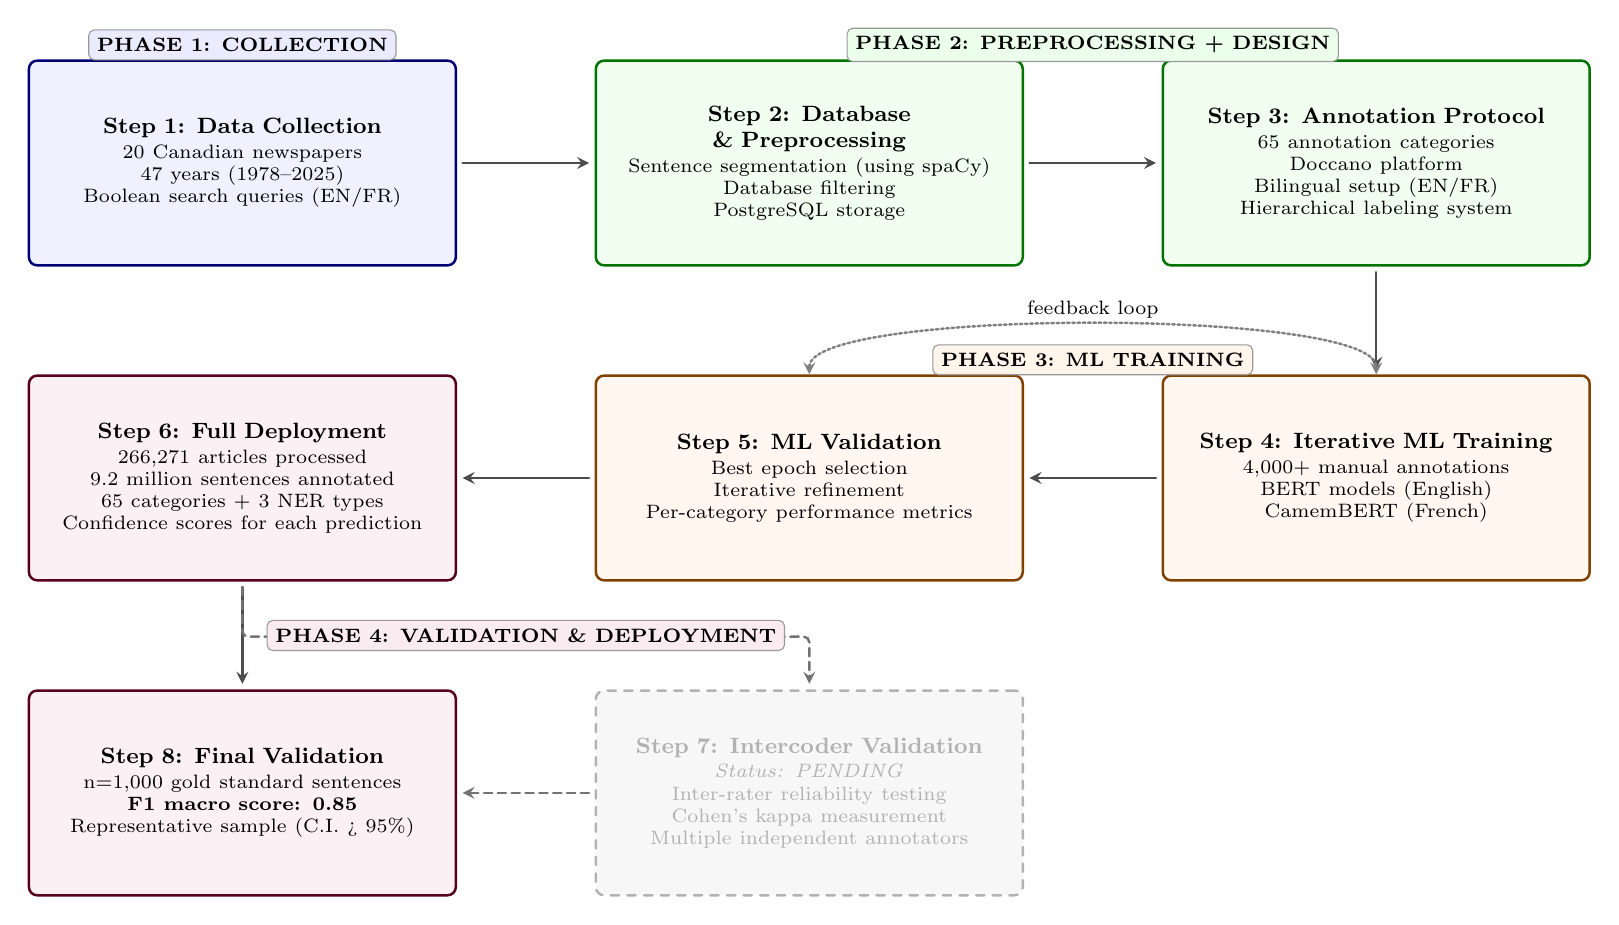
\begin{tikzpicture}[
    box/.style = {
        rectangle,
        draw=black!50,
        line width=0.9pt,
        rounded corners=3pt,
        minimum width=5.2cm,
        minimum height=2.6cm,
        align=center,
        font=\footnotesize,
        text width=5cm,
        inner sep=6pt,
        fill opacity=1
    },
    collect/.style = {box, fill=blue!6,   draw=blue!45!black},
    process/.style = {box, fill=green!6,  draw=green!45!black},
    train/.style   = {box, fill=orange!6, draw=orange!50!black},
    valid/.style   = {box, fill=purple!6, draw=purple!45!black},
    pending/.style = {box, fill=gray!6,   draw=gray!60, line width=0.9pt, dashed, text=gray!60},
    deploy/.style  = {box, fill=purple!6,    draw=purple!45!black},
    arrow/.style      = {->, line width=0.9pt, >=stealth, draw=black!70, rounded corners=2pt, shorten >=2pt, shorten <=2pt},
    dasharrow/.style  = {->, line width=0.9pt, >=stealth, draw=black!55, densely dashed, rounded corners=2pt, shorten >=2pt, shorten <=2pt},
    feedbackarrow/.style = {<->, line width=0.9pt, >=stealth, draw=black!50, densely dotted},
    phaselabel/.style = {rectangle, draw=black!40, rounded corners=2pt, inner sep=3pt, font=\scriptsize\bfseries},
    line cap=round, line join=round
]

% Define spacing
\def\hspace{7.2}
\def\vspace{4}

% Row 1: Steps 1-3
\node[collect] (datacoll) at (0,0) {
    \textbf{Step 1: Data Collection}\\[1pt]
    \scriptsize
    20 Canadian newspapers\\
    47 years (1978–2025)\\
    Boolean search queries (EN/FR)\\[1pt]
};

\node[process] (database) at (\hspace,0) {
  \textbf{Step 2: Database \& Preprocessing}\\[1pt]
  \scriptsize
  Sentence segmentation (using spaCy)\\
  Database filtering\\
  PostgreSQL storage\\[1pt]
};

\node[process] (protocol) at (2*\hspace,0) {
    \textbf{Step 3: Annotation Protocol}\\[1pt]
    \scriptsize
    65 annotation categories\\
    Doccano platform\\
    Bilingual setup (EN/FR)\\
    Hierarchical labeling system\\[1pt]
};

% Row 2: Steps 4-6 (right to left)
\node[train] (iterml) at (2*\hspace,-\vspace) {
    \textbf{Step 4: Iterative ML Training}\\[1pt]
    \scriptsize
    4,000+ manual annotations\\
    BERT models (English)\\
    CamemBERT (French)\\[1pt]
};

\node[train] (verification) at (\hspace,-\vspace) {
    \textbf{Step 5: ML Validation}\\[1pt]
    \scriptsize
    Best epoch selection\\
    Iterative refinement\\
    Per-category performance metrics\\[1pt]
};

\node[deploy] (fullannotation) at (0,-\vspace) {
    \textbf{Step 6: Full Deployment}\\[1pt]
    \scriptsize
    266,271 articles processed\\
    9.2 million sentences annotated\\
    65 categories + 3 NER types\\
    Confidence scores for each prediction\\[1pt]
};

% Row 3: Steps 7-8 (swapped positions)
\node[valid] (validation) at (0,-2*\vspace) {
    \textbf{Step 8: Final Validation}\\[1pt]
    \scriptsize
    n=1,000 gold standard sentences\\
    \textbf{F1 macro score: 0.85}\\
    Representative sample (C.I. > 95\%)\\[1pt]
};

\node[pending] (intercoder) at (\hspace,-2*\vspace) {
    \textbf{Step 7: Intercoder Validation}\\[1pt]
    \scriptsize
    \textit{Status: PENDING}\\
    Inter-rater reliability testing\\
    Cohen's kappa measurement\\
    Multiple independent annotators\\[1pt]
};

% Arrows - horizontal flow in row 1
\draw[arrow] (datacoll.east) -- (database.west);
\draw[arrow] (database.east) -- (protocol.west);

% Arrows - down from row 1 to row 2
\draw[arrow] (protocol.south) -- (iterml.north);

% Arrows - horizontal flow in row 2 (right to left)
\draw[arrow] (iterml.west) -- (verification.east);
\draw[arrow] (verification.west) -- (fullannotation.east);

% Feedback loop - properly above the boxes
% Feedback loop — connect exactly at node tops, with smooth arch
\draw[feedbackarrow]
    (verification.north) to[out=90,in=90, looseness=0.3]
    node[above, yshift=1pt, font=\scriptsize, fill=white, inner sep=1pt] {feedback loop}
    (iterml.north);

% Arrows - down to row 3
\draw[arrow] (fullannotation.south) -- (validation.north);
\draw[dasharrow] (fullannotation.south) -- ++(0,-0.7) -| (intercoder.north);
\draw[dasharrow] (intercoder.west) -- (validation.east);

% Phase labels (muted colors, clearer grouping)
\node[phaselabel, fill=blue!8]   at (0,1.5)               {PHASE 1: COLLECTION};
\node[phaselabel, fill=green!8]  at (1.5*\hspace,1.5)     {PHASE 2: PREPROCESSING + DESIGN};
\node[phaselabel, fill=orange!8] at (1.5*\hspace,-2.5)    {PHASE 3: ML TRAINING};
\node[phaselabel, fill=purple!8] at (0.5*\hspace,-1.5*\vspace)    {PHASE 4: VALIDATION \& DEPLOYMENT};

\end{tikzpicture}
}
\caption{Methodological pipeline of the Canadian Climate Framing (CCF) project.}
\label{fig:methodology_overview}
\end{figure}
\vspace*{\fill}

\end{landscape}

\subsubsection{Step 2: Preprocessing}

The preprocessing phase transformed this raw collection into a structured dataset suitable for machine learning analysis. Each article was segmented into two-sentence contexts using language-specific spaCy models\footnote{We employed en\_core\_web\_lg for English text and fr\_dep\_news\_trf for French text, both optimized for news content processing.}. Sliding windows with single-sentence overlaps were implemented to ensure complete coverage while maintaining semantic continuity throughout each article. The choice of two-sentence units was made to provide sufficient information in each segment, given the complexity of some categories we developed.

Quality control measures were applied systematically throughout the data preparation pipeline. We identified and removed duplicate articles with fuzzy string-similarity algorithms set to a 95\% threshold. This process reduced the corpus to 266,271 unique articles\footnote{We retained duplicates of the same article from different media outlets to enable the measurement of media bubbles.}. We verified language with fastText\footnote{fastText is an open-source library by Facebook AI Research for text classification and word representations; its pre-trained language identification model detects the language of a text with high accuracy. See \url{https://fasttext.cc/}.} to ensure accurate categorization of bilingual content, and we standardized dates and performed UTF-8 normalization to resolve inconsistencies that stemmed from multiple data sources. This data preparation produced a clean, standardized corpus ready for annotation, which we stored in two PostgreSQL tables: one with full metadata (including titles, main text, authors, dates, and page numbers\footnote{These metadata are very important: they enable modeling the probability of appearing on the front page and tracking coverage by individual journalists over time, among other analyses.}) and another with the processed text data (including sentence segments and their corresponding IDs).

The resulting database is illustrated in Figure~\ref{fig:media_dist}, which displays the distribution of article counts by media (20 outlets), while Figure~\ref{fig:year_counts} shows total article counts per year across the full time span (excluding 2025\footnote{Data extraction concluded in February 2025; consequently, we exclude 2025 from the yearly counts because the year is incomplete. We nevertheless plan to update the database regularly and create an observatory.}). Finally, Figure~\ref{fig:province_dist} presents the distribution of articles by province, based on the primary location of each newspaper. This geographic breakdown shows the representativeness of the database across Canada (with 17.1\% of French articles, and 82.9\% of English articles). Three national newspapers are omitted from the provincial breakdown due to their pan-Canadian scope; nevertheless, they account for 36.2\% of the articles: The Globe and Mail, the National Post, and the Toronto Star.

\begin{figure}[!htbp]
  \centering
  \begin{minipage}[c]{0.48\textwidth}
    \centering
    \includegraphics[width=\linewidth]{../Results/Outputs/Figures/articles_by_media.png}
    \caption{Distribution of articles by media.}
    \label{fig:media_dist}
      \end{minipage}
  \hspace{0.02\textwidth}
  \begin{minipage}[c]{0.48\textwidth}
    \centering
    \includegraphics[width=\linewidth]{../Results/Outputs/Figures/articles_by_year.png}
    \caption{Total number of articles per year.}
    \label{fig:year_counts}
      \end{minipage}
\end{figure}

\begin{figure}[!htbp]
  \centering
  \includegraphics[width=0.8\textwidth,keepaspectratio]{../Results/Outputs/Figures/articles_by_province.png}
  \caption{Distribution of articles by province.}
  \label{fig:province_dist}
  \end{figure}

\subsubsection{Step 3: Annotation protocol}

The annotation framework represents the conceptual foundation of the CCF database. It encompasses 65 distinct categories organized into a hierarchical taxonomy. This comprehensive system was built through iterative refinement and combines established categories from climate communication literature with novel classifications identified through exploratory analysis of the CCF Database. The framework operates at three interconnected levels: detection-level binary classification determining the presence or absence of primary categories, sub-categorization providing fine-grained classification within detected categories, and entity-level extraction identifying and classifying named entities within the text. The complete detailed taxonomy with all 65 individual categories and their operational definitions is provided in Appendix~\ref{sec:appendix} (Table~\ref{tab:complete_framework}), but in Table~\ref{tab:framework_summary} we present a summary of the framework's structure and key categories.

The annotation framework possesses four primary categories (\emph{Frames}, \emph{Actors}, \emph{Events} and \emph{Solutions}) each with their own sub-categories. Each primary category is designed to detect the presence of the overarching dimension, while its sub-categories capture the internal distinctions within that dimension. For example, the \emph{Economic Frame} is designed to categorize and detect any mention of economic aspects related to climate change, and it includes several categories that aim to capture specific economic sub-dimensions, such as negative/positive impacts of climate change on the economy, the costs and benefits of action, and economics sectors' footprint. The primary category \emph{Actors/Messengers} captures any actor or messenger that is mentioned in the text and encompasses nine sub-categories, including scientists, politicians, activists, and various types of experts (medical, economic, security, legal, cultural); and so on for the primary categories. 

The rest of the framework is composed of primary categories without sub-categories, including \emph{Emotional Tone} (Positive, Negative, Neutral/none), \emph{Geographic Focus} (Canadian location), \emph{Urgency/Alarmism} (conveying immediate danger or crisis), and \emph{Named Entities} (Persons, Organizations, Locations). These categories capture additional dimensions of climate discourse that are crucial for understanding the framing and context of climate change in Canadian media. The following real example from the database—an excerpt from a 2022 article—illustrates the corresponding manual annotations:

% Polished, self-contained example
\begin{figure}[!ht]
\centering
\fcolorbox{gray!60}{gray!5}{
  \begin{minipage}{0.96\linewidth}
    \small
    \textbf{Example (annotated sentence).}\\[0.3em]
    \emph{``In Scientific American, professor of Environmental Studies at Humboldt State University Sarah Jaquette Ray writes, `Climate anxiety can operate like white fragility, sucking up all the oxygen in the room and devoting resources toward appeasing the dominant group.' But it would be a mistake to conclude that this term isn't applicable in the Global South, period.''}\\[0.6em]
    \begin{tabularx}{\linewidth}{@{}lX@{}}
      \toprule
      \textbf{Dimension} & \textbf{Tagged categories} \\
      \midrule
      Actors & Scientists \\
      Thematic frames & Justice (primary category) + North--South responsibility; Health (primary category) \\
      Emotional tone & Negative emotion (anxiety) \\
      \bottomrule
    \end{tabularx}
  \end{minipage}
}
\end{figure}

\begin{table}[!ht]
\centering
\caption{The CCF annotation framework: 65 hierarchical categories for comprehensive climate discourse analysis}
\label{tab:framework_summary}
\footnotesize
\begin{tabularx}{\textwidth}{lcX}
\toprule
\rowcolor{gray!15}
\textbf{Main Category} & \textbf{N}$^a$ & \textbf{Sub-categories and Detection Elements} \\
\midrule
\multicolumn{3}{l}{\cellcolor{gray!10}\textbf{\textit{Primary Categories: Thematic Frames (8 frames with 35 sub-categories)}}} \\
\midrule
\textbf{Economic} & 6 & Negative/positive impacts, costs/benefits of action, sector footprint, general link \\
\textbf{Health} & 5 & Negative/positive impacts, co-benefits, healthcare footprint, general link \\
\textbf{Security} & 5 & Military response, base disruption, displacement, conflicts, defense footprint \\
\textbf{Justice} & 5 & Winners/losers, North-South responsibility, legitimacy, litigation, general link \\
\textbf{Political} & 3 & Policy measures, political debate \& opinion, general link \\
\textbf{Scientific} & 3 & Controversy, discovery \& innovation, general link \\
\textbf{Environmental} & 3 & Habitat loss, species loss, general biodiversity link \\
\textbf{Cultural} & 5 & Art, events, Indigenous practices, cultural footprint, general link \\
\midrule
\multicolumn{3}{l}{\cellcolor{gray!10}\textbf{\textit{Primary Categories: Actors, Events and Solutions (with 15 sub-categories)}}} \\
\midrule
\textbf{Actors/Messengers} & 9 & Scientists, politicians, activists, medical/economic/security/legal/cultural experts, any messenger \\
\textbf{Events} & 6 & Natural disasters, conferences, reports, elections, policy announcements, any event \\
\textbf{Solutions} & 3 & Mitigation, adaptation, any solution mention \\
\midrule
\cellcolor{gray!10}\textbf{Emotional Tone} & \cellcolor{gray!10}3 & \cellcolor{gray!10}Positive (hope, optimism), Negative (fear, anxiety), Neutral/none \\
\midrule
\cellcolor{gray!10}\textbf{Geographic Focus} & \cellcolor{gray!10}1 & \cellcolor{gray!10}Canadian places, actors, data, and policies \\
\midrule
\cellcolor{gray!10}\textbf{Urgency/Alarmism} & \cellcolor{gray!10}1 & \cellcolor{gray!10}Conveys immediate danger, crisis, or ``code red'' urgency \\
\midrule
\cellcolor{gray!10}\textbf{Named Entities} & \cellcolor{gray!10}3 & \cellcolor{gray!10}Persons (PER), Organizations (ORG), Locations (LOC) \\
\midrule
\multicolumn{3}{l}{\cellcolor{gray!25}\textbf{Total: 65 categories}} \\
\bottomrule
\end{tabularx}
\vspace{-0.1em}
{\footnotesize $^a$The \emph{N} count includes detection of the main category plus its sub-categories. For example: Economic frame detection + 5 sub-categories = 6.}
\end{table}

\subsection{Phase 3: Machine learning}
\subsubsection{Step 4 \& 5: Iterative machine learning training and validation}

The development of training data followed an iterative manual annotation protocol aligned with the annotation framework previously described. A single expert annotator (climate policy and communication) labeled sentences in sequential batches (first 2,000 sentences, then three additional batches of 1,000 each) for a total of 4,000 annotated samples. The batching served two explicit objectives: (1) to iteratively improve and stabilize the annotation guidelines after each round; and (2) to progressively monitor and optimize model training to reach the highest attainable F1 score. This process culminated in a macro F1 score of 0.826 (see Table~\ref{tab:performance}) during the training phase (see Table~\ref{tab:complete_training_metrics} in Appendix~\ref{sec:appendix} for detailed metrics).

The sampling process drew equally from English and French language groups, with final annotation counts reaching 1,927 English and 2,073 French sentences. The training dataset was subsequently partitioned using stratified random sampling to create training (80\%) and validation (20\%) databases for each category and language. Table~\ref{tab:training_distribution} in Appendix~\ref{sec:appendix} provides the complete distribution of training and validation samples for all annotation categories \autocite{doAugmentedSocialScientist2022}. The random sampling approach ensured broad coverage across the temporal span and diverse media sources. While inter-annotator reliability assessment is in progress with a second coder, the annotation protocol was developed with detailed operational definitions for each of the 65 categories to ensure consistency.

The machine learning pipeline leveraged state-of-the-art transformer architectures optimized for each language through a custom fork of the AugmentedSocialScientist library \autocite{doAugmentedSocialScientist2022,lemorAntoinelemorAugmentedSocialScientistFork2025}. The fork we built from \textcite{doAugmentedSocialScientist2022} add several functionnalities that are central to ensure robust machine learning training. The fork provides: metric logging at every training epoch, intelligent best-model selection using a weighted F1 score (0.7 × F1-positive + 0.3 × macro-F1), automatic device optimization, and an automated reinforced training protocol for underperforming models (described below) \autocite{lemorAntoinelemorAugmentedSocialScientistFork2025}. English text processing employed BERT-base-uncased, while French text utilized CamemBERT-base, both containing 110 million parameters. The training strategy implemented hierarchical classification, where detection models were trained first as binary classifiers on the full annotated dataset, followed by sub-classification models trained exclusively on manually annotated sentences that were positive for the corresponding primary category. This approach minimized false positive propagation and allowed for specialized optimization for each classification task.

\begin{table}[b!]
\centering
\caption{Model training performance metrics for primary annotation categories}
\label{tab:performance}
\small
\begin{tabular}{l|rr|rr|rr}
\toprule
\rowcolor{gray!10}
\textbf{Category} & \multicolumn{2}{c}{\textbf{F1 (Class 1)}} & \multicolumn{2}{c}{\textbf{F1 (Class 0)}} & \multicolumn{2}{c}{\textbf{Macro F1}} \\
\cline{2-7}
\rowcolor{gray!10}
& \textbf{EN} & \textbf{FR} & \textbf{EN} & \textbf{FR} & \textbf{EN} & \textbf{FR} \\
\midrule
\rowcolor{gray!10}
\multicolumn{7}{l}{\textit{Thematic Frames}} \\
\midrule
Economic Frame & 0.745 & 0.814 & 0.944 & 0.957 & 0.845 & 0.885 \\
Health Frame & 0.800 & 0.667 & 0.989 & 0.994 & 0.894 & 0.830 \\
Security Frame & 0.870 & 0.800 & 0.996 & 0.997 & 0.933 & 0.898 \\
Justice Frame & 0.719 & 0.717 & 0.975 & 0.981 & 0.847 & 0.849 \\
Political Frame & 0.808 & 0.774 & 0.897 & 0.888 & 0.853 & 0.831 \\
Scientific Frame & 0.784 & 0.702 & 0.953 & 0.962 & 0.869 & 0.832 \\
Environmental Frame & 0.842 & 0.625 & 0.989 & 0.980 & 0.915 & 0.802 \\
Cultural Frame & 0.773 & 0.833 & 0.986 & 0.993 & 0.879 & 0.913 \\
\midrule
\rowcolor{gray!10}
\multicolumn{7}{l}{\textit{Other Primary Categories: Actors, Events and Solutions}} \\
\midrule
Actors/Messengers Detection & 0.912 & 0.929 & 0.904 & 0.915 & 0.908 & 0.922 \\
Event Detection & 0.794 & 0.819 & 0.935 & 0.932 & 0.865 & 0.876 \\
Solutions Detection & 0.737 & 0.878 & 0.914 & 0.944 & 0.825 & 0.911 \\
Canadian Context & 0.942 & 0.964 & 0.968 & 0.980 & 0.955 & 0.972 \\
Urgency/Alarmism & 0.760 & 0.690 & 0.987 & 0.981 & 0.874 & 0.835 \\
\midrule
\rowcolor{gray!15}
\textbf{Overall Average}* & \textbf{0.769} & \textbf{0.739} & \textbf{0.905} & \textbf{0.909} & \textbf{0.837} & \textbf{0.816} \\
\rowcolor{gray!15}
\textbf{Combined (ALL)} & \multicolumn{2}{c}{\textbf{0.754}} & \multicolumn{2}{c}{\textbf{0.907}} & \multicolumn{2}{c}{\textbf{0.826}} \\
\bottomrule
\end{tabular}

\vspace{0.3em}
\noindent\footnotesize
*Overall average across all active annotation categories (see Table~\ref{tab:complete_training_metrics} for complete metrics).
\end{table}

Models failing to achieve positive-class F1 scores above 0.70 during the training phase underwent an automated reinforced training protocol\footnote{This protocol was necessary for 15 underperforming models, primarily in abstract conceptual categories such as cultural and justice sub-frames.}. The reinforced phase implemented weighted random sampling to oversample minority classes, doubled batch size to 64, reduced learning rate to 1e-5, and applied weighted cross-entropy loss with emphasis on the positive class. This reinforcement protocol, extending training for an additional 20 epochs, successfully improved mean F1 scores by 0.23 across affected models, and managed to bring most categories above the acceptable performance threshold.

However, five categories could not be trained due to insufficient annotations in the training data and were consequently excluded from the annotation framework: carbon footprint of the health sector, positive health impacts of climate change, military disaster response, climate impacts on military operations, and carbon footprint of the security sector. These categories are not represented in the performance metrics table (Table~\ref{tab:performance}).

\subsection{Phase 4: Validation \& Deployment}

\subsubsection{Step 6: Full Deployment}

The full deployment phase applied all the trained models to annotate the complete CCF Database of 9.2 million sentences across 266,271 articles. We implemented a hierarchical classification strategy that directly mirrors the annotation protocol's structure of primary categories and their associated sub-categories, as illustrated in Figure~\ref{fig:hierarchical_annotation}. 

The hierarchical approach reflects the conceptual organization of our annotation framework with eleven primary detection categories, each with specific sub-categories. The eight thematic frames (\emph{Economic}, \emph{Health}, \emph{Security}, \emph{Justice}, \emph{Political}, \emph{Scientific}, \emph{Environmental}, and \emph{Cultural Frame Detection}) function as primary categories with their internal distinctions—for example, \emph{Economic Frame Detection}, when positive (=1), triggers six economic sub-models (\emph{Negative/Positive Economic Impacts}, \emph{Costs/Benefits of Climate Action}, \emph{Economic Sector Footprint}), while a negative detection (=0) bypasses these entirely. 

\begin{figure}[b!]
\centering
\resizebox{0.95\textwidth}{!}{%
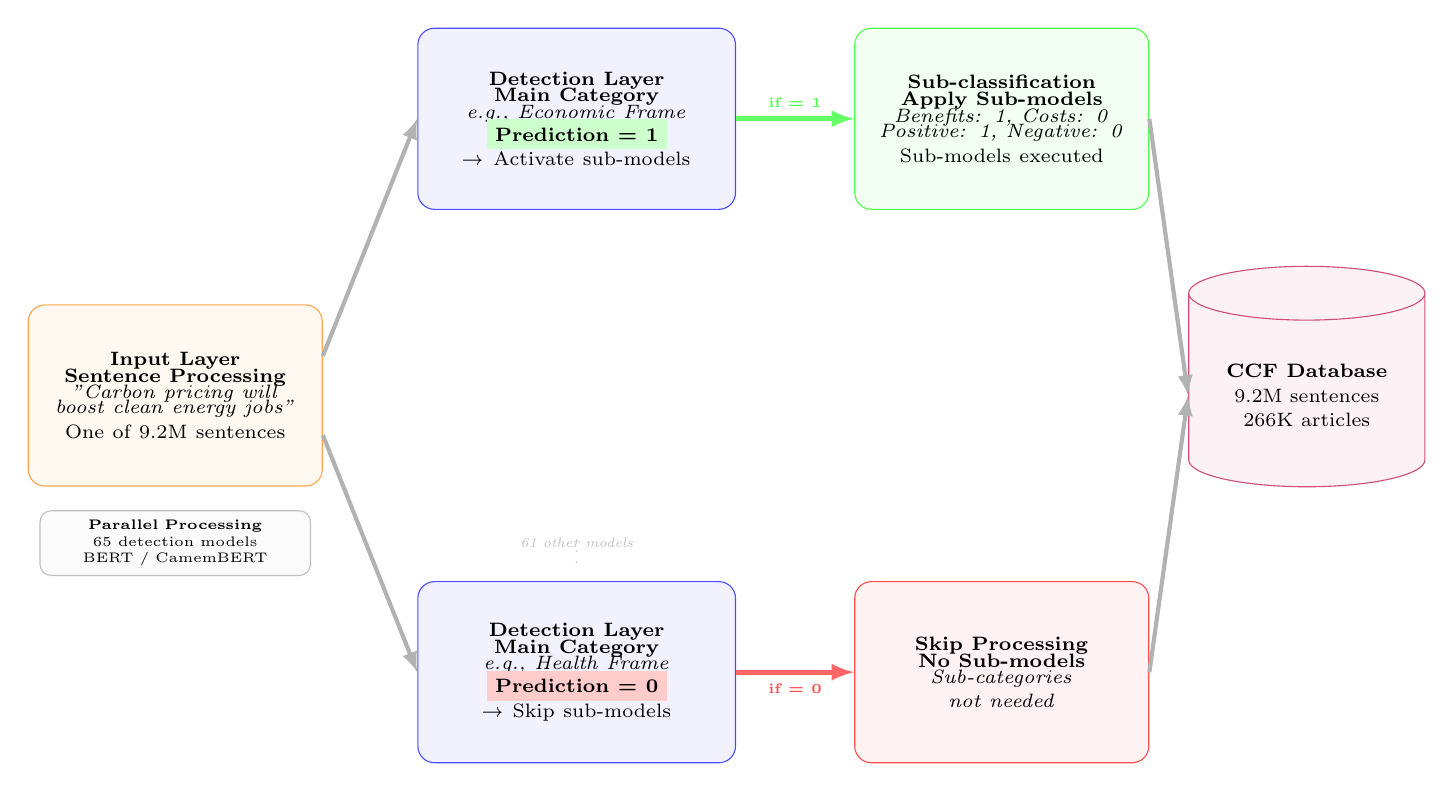
\begin{tikzpicture}[
    % Style definitions with reduced widths
    stage/.style={rectangle, rounded corners=6pt, minimum height=2.3cm, text width=3.8cm, align=center, font=\small},
    input/.style={stage, draw=orange!70, fill=orange!5, text width=3.5cm},
    detect/.style={stage, draw=blue!70, fill=blue!5, text width=3.8cm},
    process/.style={stage, draw=green!70, fill=green!5, text width=3.5cm},
    skip/.style={stage, draw=red!70, fill=red!5, text width=3.5cm},
    storage/.style={cylinder, draw=purple!70, fill=purple!5, shape border rotate=90, minimum height=2.8cm, minimum width=3cm, align=center, font=\small, aspect=0.3},
    arrow/.style={->, >=latex, line width=1.5pt, color=gray!60},
    yes/.style={arrow, color=green!60},
    no/.style={arrow, color=red!60},
    label/.style={font=\tiny\bfseries}
]

% Stage 1: Input
\node[input] (input) {
    \scriptsize\textbf{Input Layer}\\[-2pt]
    \scriptsize\textbf{Sentence Processing}\\[-2pt]
    \textit{\scriptsize "Carbon pricing will}\\[-2.5pt]
    \textit{\scriptsize boost clean energy jobs"}\\[-2pt]
    \scriptsize{One of 9.2M sentences}
};

% Stage 2: Detection (parallel branches)
\node[detect, above right=1.2cm and 1.2cm of input] (detect_yes) {
    \scriptsize\textbf{Detection Layer}\\[-2pt]
    \scriptsize\textbf{Main Category}\\[-2pt]
    \textit{\scriptsize e.g., Economic Frame}\\[-2pt]
    \colorbox{green!20}{\scriptsize\textbf{Prediction = 1}}\\[-2pt]
    \scriptsize{→ Activate sub-models}
};

\node[detect, below right=1.2cm and 1.2cm of input] (detect_no) {
    \scriptsize\textbf{Detection Layer}\\[-2pt]
    \scriptsize\textbf{Main Category}\\[-2pt]
    \textit{\scriptsize e.g., Health Frame}\\[-2pt]
    \colorbox{red!20}{\scriptsize\textbf{Prediction = 0}}\\[-2pt]
    \scriptsize{→ Skip sub-models}
};

% Stage 3: Conditional execution
\node[process, right=1.5cm of detect_yes] (execute) {
    \scriptsize\textbf{Sub-classification}\\[-2pt]
    \scriptsize\textbf{Apply Sub-models}\\[-2pt]
    \textit{\scriptsize Benefits: 1, Costs: 0}\\[-2.5pt]
    \textit{\scriptsize Positive: 1, Negative: 0}\\[-2pt]
    \scriptsize{Sub-models executed}
};

\node[skip, right=1.5cm of detect_no] (bypass) {
    \scriptsize\textbf{Skip Processing}\\[-2pt]
    \scriptsize\textbf{No Sub-models}\\[-2pt]
    \textit{\scriptsize Sub-categories}\\[-2.5pt]
    \textit{\scriptsize not needed}
};

% Stage 4: Storage - positioned at center between execute and bypass
\node[storage] (database) at ($(execute.east)!0.5!(bypass.east) + (2cm,0)$) {
    \scriptsize\textbf{CCF Database}\\[-2pt]
    \scriptsize 9.2M sentences\\[-2.5pt]
    \scriptsize 266K articles
};

% Connections
\draw[arrow] (input.15) -- (detect_yes.west);
\draw[arrow] (input.-15) -- (detect_no.west);

\draw[yes, line width=1.8pt] (detect_yes) -- node[above, label] {\textcolor{green!70}{if = 1}} (execute);
\draw[no, line width=1.8pt] (detect_no) -- node[below, label] {\textcolor{red!70}{if = 0}} (bypass);

\draw[arrow] (execute.east) -- (database.west);
\draw[arrow] (bypass.east) -- (database.west);

% Architecture info box
\node[below=0.3cm of input, draw=gray!50, fill=gray!3, rounded corners=4pt, text width=3.2cm, align=center, font=\tiny] {
    \textbf{Parallel Processing}\\
    65 detection models\\
    BERT / CamemBERT
};

% Visual indicator for parallel processing - better positioned
\node[above=0.3cm of detect_no, font=\tiny\itshape, text=gray!50] {61 other models};
\node[above=0.1cm of detect_no, font=\tiny, text=gray!50] {$\vdots$};

\end{tikzpicture}
}
\caption{Hierarchical annotation pipeline. The system processes each sentence through detection models that determine whether corresponding sub-category models should be applied, enabling efficient annotation of the entire corpus.}
\label{fig:hierarchical_annotation}
\end{figure}

Similarly, the three other primary categories follow this conditional logic: \emph{Actors/Messengers Detection} activates nine actor-type sub-models (\emph{Health Expert}, \emph{Economic Expert}, \emph{Security Expert}, \emph{Legal Expert}, \emph{Cultural Expert}, \emph{Natural Scientist}, \emph{Social Scientist}, \emph{Activist}, \emph{Public Official}), \emph{Event Detection} triggers eight event-type classifications (\emph{Extreme Weather Event}, \emph{Meeting/Conference}, \emph{Publication}, \emph{Election}, \emph{Policy Announcement}, \emph{Judiciary Decision}, \emph{Cultural Event}, \emph{Protest}), and \emph{Solutions Detection} applies two solution sub-categories (\emph{Mitigation Strategy}, \emph{Adaptation Strategy}). The deployment also processed standalone primary categories without hierarchical structure—\emph{Emotional Tone} (\emph{Positive Emotion}/\emph{Negative Emotion}/\emph{Neutral Emotion}), \emph{Geographic Focus} (\emph{Canadian Context}), \emph{Urgency/Alarmism}. 

\begin{figure}[b!]
\centering
\resizebox{0.70\linewidth}{!}{%
\iffalse % Disable complex original diagram (replaced by compact version below)
\begin{tikzpicture}[
    % Style definitions (muted, consistent, readable)
    header/.style={rectangle, draw=black!50, fill=gray!10, minimum width=3cm, minimum height=0.8cm, align=center, font=\footnotesize\bfseries},
    metadata/.style={rectangle, draw=gray!50, fill=gray!6, minimum width=2.2cm, minimum height=0.6cm, align=center, font=\scriptsize},
    frame/.style={rectangle, draw=green!45!black, fill=green!6, minimum width=1.8cm, minimum height=0.6cm, align=center, font=\scriptsize\itshape},
    actor/.style={rectangle, draw=blue!45!black,  fill=blue!6,  minimum width=1.8cm, minimum height=0.6cm, align=center, font=\scriptsize\itshape},
    event/.style={rectangle, draw=cyan!50!black,  fill=cyan!6,  minimum width=1.8cm, minimum height=0.6cm, align=center, font=\scriptsize\itshape},
    solution/.style={rectangle, draw=teal!50!black, fill=teal!6, minimum width=1.8cm, minimum height=0.6cm, align=center, font=\scriptsize\itshape},
    other/.style={rectangle, draw=purple!45!black, fill=purple!6, minimum width=1.8cm, minimum height=0.6cm, align=center, font=\scriptsize\itshape},
    subcategory/.style={rectangle, draw=orange!60!black, fill=orange!6, minimum width=1.6cm, minimum height=0.5cm, align=center, font=\scriptsize},
    example_box/.style={rectangle, rounded corners=6pt, draw=black!30, fill=gray!4, minimum width=14cm, minimum height=2cm, align=left, font=\scriptsize},
    legend/.style={rectangle, draw=black!30, fill=white, align=left, font=\scriptsize, rounded corners=3pt, inner sep=4pt},
    arrow/.style={->, >=Stealth, line width=0.9pt, draw=black!65},
    group_box/.style={draw=black!25, rounded corners=3pt, inner sep=6pt, fill=black!2},
    line cap=round, line join=round
]

% Database table header
\node[header] (table_header) at (0,0) {The CCF Database: CCF\_processed\_data (9.2M sentences × 71 columns)};

% Metadata columns (horizontally arranged)
\node[metadata, below=0.4cm of table_header, xshift=-7cm] (doc_id) {Article ID};
\node[metadata, right=0.05cm of doc_id] (sent_id) {Sentence ID};
\node[metadata, right=0.05cm of sent_id] (sentence) {Sentence Text};
\node[metadata, right=0.05cm of sentence] (lang) {Language};
\node[metadata, right=0.05cm of lang] (date) {Date};
\node[metadata, right=0.05cm of date] (media) {Media};

% PRIMARY CATEGORIES WITH SUB-CATEGORIES (vertically stacked)
% Frames (8 categories)
\node[frame, below=1cm of table_header, xshift=-3cm] (eco_frame) {Economic Frame};
\node[frame, right=0.05cm of eco_frame] (health_frame) {Health Frame};
\node[frame, right=0.05cm of health_frame] (security_frame) {Security Frame};
\node[frame, right=0.05cm of security_frame] (justice_frame) {Justice Frame};

\node[frame, below=0.05cm of eco_frame] (pol_frame) {Political Frame};
\node[frame, right=0.05cm of pol_frame] (sci_frame) {Scientific Frame};
\node[frame, right=0.05cm of sci_frame] (env_frame) {Environmental Frame};
\node[frame, right=0.05cm of env_frame] (cult_frame) {Cultural Frame};

% Actors/Messengers
\node[actor, below=0.8cm of pol_frame, xshift=0cm] (messenger) {Actors/Messengers Detection};
\node[actor, right=0.05cm of messenger] (scientist) {Scientists};
\node[actor, right=0.05cm of scientist] (politician) {Politicians};
\node[actor, right=0.05cm of politician] (activist) {Activists};

\node[actor, below=0.05cm of messenger] (medical) {Medical Experts};
\node[actor, right=0.05cm of medical] (economic) {Economic Experts};
\node[actor, right=0.05cm of economic] (security) {Security Experts};
\node[actor, right=0.05cm of security] (legal) {Legal Experts};

% Events  
\node[event, below=0.8cm of medical, xshift=0cm] (event_det) {Event Detection};
\node[event, right=0.05cm of event_det] (disaster) {Natural Disasters};
\node[event, right=0.05cm of disaster] (conference) {Climate Conferences};
\node[event, right=0.05cm of conference] (report) {Report Releases};

% Solutions
\node[solution, below=0.05cm of event_det] (solution_det) {Solutions Detection};
\node[solution, right=0.05cm of solution_det] (mitigation) {Mitigation Strategies};
\node[solution, right=0.05cm of mitigation] (adaptation) {Adaptation Strategies};

% OTHER PRIMARY CATEGORIES (no sub-categories)
\node[other, below=1cm of table_header, xshift=4.5cm] (emotion_neg) {Negative Emotion};
\node[other, right=0.05cm of emotion_neg] (emotion_pos) {Positive Emotion};
\node[other, right=0.05cm of emotion_pos] (emotion_neutral) {Neutral Emotion};

\node[other, below=0.05cm of emotion_neg] (canadian) {Canadian Context};
\node[other, right=0.05cm of canadian] (urgency) {Urgency/Alarmism};

\node[other, below=0.05cm of canadian] (ner_per) {Person (NER)};
\node[other, right=0.05cm of ner_per] (ner_org) {Organization (NER)};
\node[other, right=0.05cm of ner_org] (ner_loc) {Location (NER)};

% SUB-CATEGORIES (examples)
\node[subcategory, below=0.3cm of eco_frame, xshift=-0.5cm] (eco_sub1) {\scriptsize Negative Impacts};
\node[subcategory, right=0.02cm of eco_sub1] (eco_sub2) {\scriptsize Costs of Action};
\node[font=\tiny, right=0.02cm of eco_sub2] {...4 more};

\node[subcategory, below=0.3cm of event_det, xshift=-0.5cm] (event_sub1) {\scriptsize Election};
\node[subcategory, right=0.02cm of event_sub1] (event_sub2) {\scriptsize Policy Announce.};
\node[font=\tiny, right=0.02cm of event_sub2] {...};

% Group boxes with labels (improves structure and readability)
\node[group_box, fit=(doc_id)(sent_id)(sentence)(lang)(date)(media),
      label={[anchor=north west, yshift=2pt, xshift=2pt, font=\scriptsize\bfseries, text=gray!70]north west:Metadata (6 cols)}] (grp_meta) {};

\node[group_box, fit=(eco_frame)(health_frame)(security_frame)(justice_frame)(pol_frame)(sci_frame)(env_frame)(cult_frame)(eco_sub1)(eco_sub2),
      label={[anchor=north west, yshift=2pt, xshift=2pt, font=\scriptsize\bfseries, text=green!60]north west:Frames (8 primary + subs)}] (grp_frames) {};

\node[group_box, fit=(messenger)(scientist)(politician)(activist)(medical)(economic)(security)(legal),
      label={[anchor=north west, yshift=2pt, xshift=2pt, font=\scriptsize\bfseries, text=blue!60]north west:Actors/Messengers (9 cols)}] (grp_actors) {};

\node[group_box, fit=(event_det)(disaster)(conference)(report)(event_sub1)(event_sub2),
      label={[anchor=north west, yshift=2pt, xshift=2pt, font=\scriptsize\bfseries, text=cyan!60]north west:Events (6 cols)}] (grp_events) {};

\node[group_box, fit=(solution_det)(mitigation)(adaptation),
      label={[anchor=north west, yshift=2pt, xshift=2pt, font=\scriptsize\bfseries, text=teal!60]north west:Solutions (3 cols)}] (grp_solutions) {};

\node[group_box, fit=(emotion_neg)(emotion_pos)(emotion_neutral)(canadian)(urgency)(ner_per)(ner_org)(ner_loc),
      label={[anchor=north west, yshift=2pt, xshift=2pt, font=\scriptsize\bfseries, text=purple!60]north west:Other Primary (8 cols)}] (grp_other) {};

% Legend (top-right)
\node[legend, right=0.8cm of table_header, anchor=north west] (legendbox) {
    \textbf{Legend}\\[-1pt]
    {\color{gray!60}\rule{6pt}{6pt}}\; Metadata\\
    {\color{green!60}\rule{6pt}{6pt}}\; Frames\\
    {\color{blue!60}\rule{6pt}{6pt}}\; Actors\\
    {\color{cyan!60}\rule{6pt}{6pt}}\; Events\\
    {\color{teal!60}\rule{6pt}{6pt}}\; Solutions\\
    {\color{purple!60}\rule{6pt}{6pt}}\; Other
};

% Hierarchical arrows (examples)
\draw[arrow] (eco_frame.south) -- (eco_sub1.north);
\draw[arrow] (event_det.south) -- (event_sub1.north);

% Example with 4 sentences from same article
\node[example_box, below=5.5cm of table_header, minimum width=16cm, minimum height=2.8cm] (example) {
    \textbf{Example: Article A2019-042 (The Globe and Mail, 2019-07-15)}\\[3pt]
    \begin{tabular}{|c|c|p{5cm}|c|p{1.8cm}|p{2.8cm}|}
    \hline
    \textbf{ID} & \textbf{Sent} & \textbf{Text} & \textbf{Lang} & \textbf{Primary} & \textbf{Sub-categories} \\
    \hline
    042 & 1 & ``Climate scientists warn that economic disruption...'' & EN & Econ=1, Mess=1 & Negative Impacts=1 \\
    042 & 2 & ``The government announced sweeping new measures...'' & EN & Pol=1, Event=1 & Policy Measures=1 \\
    042 & 3 & ``These policies will create thousands of green jobs...'' & EN & Econ=1, Sol=1 & Positive Impacts=1 \\
    042 & 4 & ``Critics worry about the cost to taxpayers...'' & EN & Econ=1, Pol=1 & Costs of Action=1 \\
    \hline
    \end{tabular}\\[3pt]
    \textit{Note: Each row = one sentence. Binary annotations (0/1) across 71 columns total.}
};

\end{tikzpicture}
\fi

% Simplified compact version (small, compile-safe)
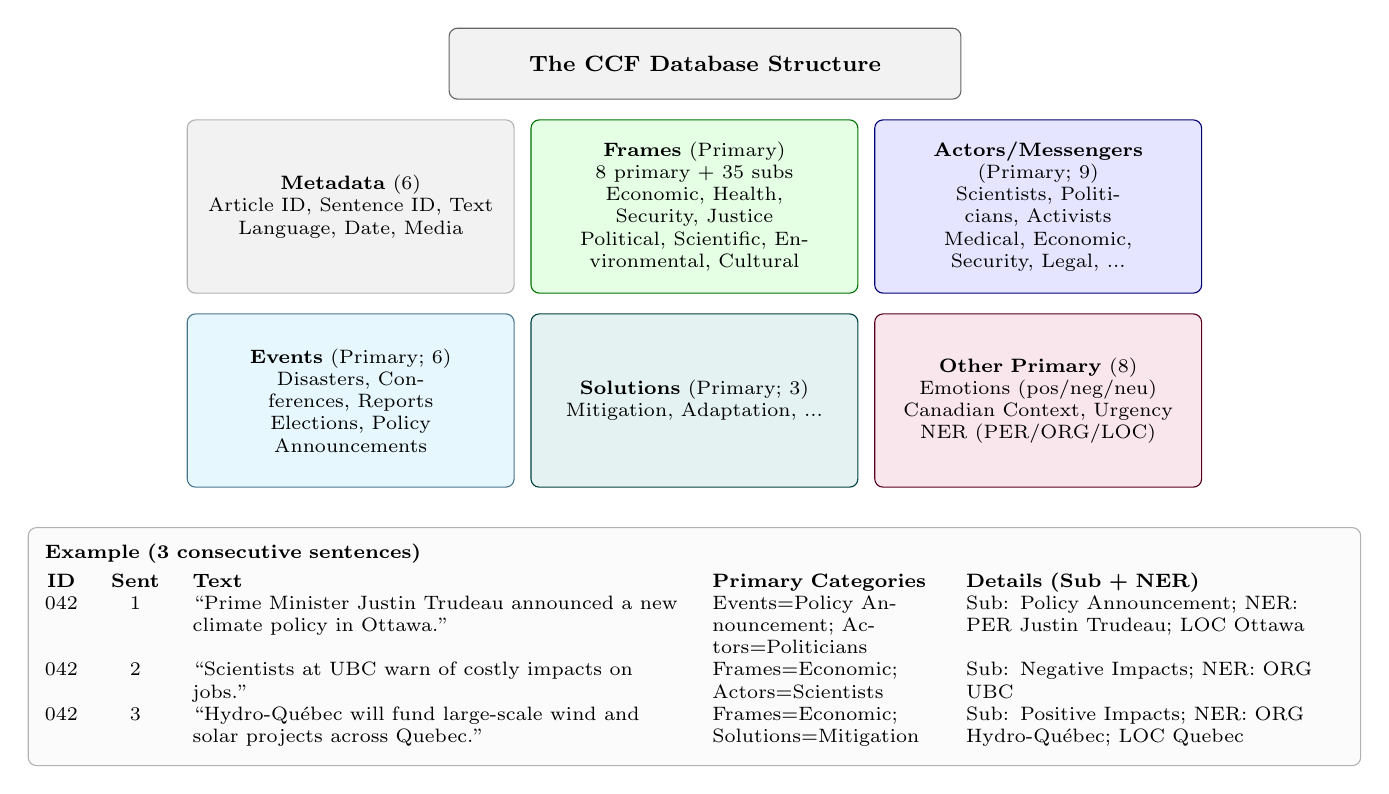
\begin{tikzpicture}[
    node distance=0.25cm and 0.2cm,
    header/.style={rectangle, draw=black!60, rounded corners=3pt, fill=gray!10, minimum width=6.5cm, minimum height=0.9cm, align=center, font=\footnotesize\bfseries},
    group/.style={rectangle, rounded corners=3pt, minimum width=4.0cm, minimum height=2.2cm, align=center, font=\scriptsize, text width=3.8cm, inner sep=5pt},
    group_meta/.style={group, draw=gray!60,   fill=gray!10},
    group_frames/.style={group, draw=green!45!black,  fill=green!10},
    group_actors/.style={group, draw=blue!45!black,   fill=blue!10},
    group_events/.style={group, draw=cyan!50!black,   fill=cyan!10},
    group_solutions/.style={group, draw=teal!50!black, fill=teal!10},
    group_other/.style={group, draw=purple!45!black,  fill=purple!10},
    example/.style={rectangle, draw=black!30, rounded corners=3pt, fill=gray!3, align=left, font=\scriptsize, text width=16.5cm, inner sep=6pt}
]

\node[header] (head) {The CCF Database Structure};

% Row 1 (three groups)
\node[group_meta, below=of head, xshift=-4.5cm] (meta) {\textbf{Metadata} (6)\\Article ID, Sentence ID, Text\\Language, Date, Media};
\node[group_frames, right=of meta] (frames) {\textbf{Frames} (Primary)\\8 primary + 35 subs\\Economic, Health, Security, Justice\\Political, Scientific, Environmental, Cultural};
\node[group_actors, right=of frames] (actors) {\textbf{Actors/Messengers} (Primary; 9)\\Scientists, Politicians, Activists\\Medical, Economic, Security, Legal, ...};

% Row 2 (three groups)
\node[group_events, below=of meta] (events) {\textbf{Events} (Primary; 6)\\Disasters, Conferences, Reports\\Elections, Policy Announcements};
\node[group_solutions, right=of events] (solutions) {\textbf{Solutions} (Primary; 3)\\Mitigation, Adaptation, ...};
\node[group_other, right=of solutions] (other) {\textbf{Other Primary} (8)\\Emotions (pos/neg/neu)\\Canadian Context, Urgency\\NER (PER/ORG/LOC)};

% Small example (simplified)
% Place the example below the second row, with extra spacing to avoid overlap
\node[example, below=0.5cm of solutions] (example) {
    \textbf{Example (3 consecutive sentences)}\\[2pt]
    \begin{tabularx}{\linewidth}{@{}c c X p{2.8cm} p{4.8cm}@{}}
    \textbf{ID} & \textbf{Sent} & \textbf{Text} & \textbf{Primary Categories} & \textbf{Details (Sub + NER)} \\
    042 & 1 & ``Prime Minister Justin Trudeau announced a new climate policy in Ottawa.'' & Events=Policy Announcement; Actors=Politicians & Sub: Policy Announcement; NER: PER Justin Trudeau; LOC Ottawa \\
    042 & 2 & ``Scientists at UBC warn of costly impacts on jobs.'' & Frames=Economic; Actors=Scientists & Sub: Negative Impacts; NER: ORG UBC \\
    042 & 3 & ``Hydro-Québec will fund large-scale wind and solar projects across Quebec.'' & Frames=Economic; Solutions=Mitigation & Sub: Positive Impacts; NER: ORG Hydro-Québec; LOC Quebec \\
    \end{tabularx}
};

\end{tikzpicture}
}
\caption{The CCF database structure (synthesized view) stores 9.2 million sentences and 71 boolean columns grouped into six families: Metadata, Frames (8 frames with 35 sub-categories), Actors/Messengers (with its subcategories), Events (with its subcategories), Solutions (with its subcategories), and other primary categories (Emotional tone, Geographic Focus, Urgence/alarmism, NER).}
\label{fig:database_structure}
\end{figure}

In addition to the custom-trained classification models, we employed pre-trained Named Entity Recognition (NER) models, selected based on empirical evaluation for optimal performance on our dataset. We implemented a hybrid approach tailored to each language: for English texts, we used BERT-base-NER\footnote{Available at: \url{https://huggingface.co/dslim/bert-base-NER}} for all three entity types (Person, Organization, Location), while for French texts, we combined spaCy's fr\_core\_news\_lg model\footnote{Available at: \url{https://spacy.io/models/fr}} for person entities with CamemBERT-NER\footnote{Available at: \url{https://huggingface.co/Jean-Baptiste/camembert-ner}} for organization and location entities. This hybrid strategy was used to leverage the respective strengths of each model: spaCy's superior performance on French person names and CamemBERT-NER's robust identification of French organizational and geographical entities (see Table~\ref{tab:ner_performance} in the Appendix for performance metrics).

The resulting CCF database structure, illustrated in Figure~\ref{fig:database_structure}, organizes the annotations in a relational PostgreSQL schema. Each sentence in the database maintains its connection to the source article metadata (publication, date, author) while storing the 65 annotation predictions as indexed boolean columns (or JSON for NER entities). The database design supports complex multi-dimensional analyses. Researchers can, for instance, query all sentences between 2015-2020 that contain economic frames with positive emotions and mention specific political actors (or even specific named entities such as Justin Trudeau).

\subsubsection{Step 7 \& 8: Final validation and inter-coder reliability}

\begin{figure}[b!]
\centering
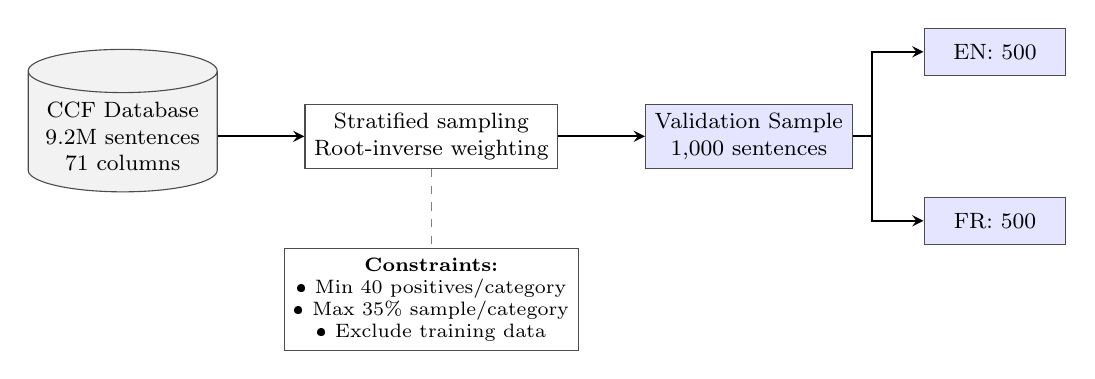
\begin{tikzpicture}[
    box/.style={rectangle, draw=black!70, fill=white, minimum width=2.2cm, minimum height=0.65cm, align=center, font=\footnotesize},
    database/.style={cylinder, draw=black!70, fill=gray!10, minimum width=2.4cm, minimum height=1cm, align=center, shape border rotate=90, aspect=0.25, font=\footnotesize},
    sample/.style={rectangle, draw=black!70, fill=blue!10, minimum width=1.8cm, minimum height=0.6cm, align=center, font=\footnotesize},
    arrow/.style={->, >=stealth, thick},
    node distance=1.1cm
]

% Centered positioning - starting at x=-3.5 for better centering
% Database (left)
\node[database] (db) at (-3.2,0) {\footnotesize CCF Database\\\footnotesize 9.2M sentences\\\footnotesize 71 columns};

% Sampling process (center-left)
\node[box, right=of db] (sampling) {\footnotesize Stratified sampling\\\footnotesize Root-inverse weighting};
\draw[arrow] (db.east) -- (sampling.west);

% Validation sample (center-right)
\node[sample, right=of sampling] (val) {\footnotesize Validation Sample\\\footnotesize 1,000 sentences};
\draw[arrow] (sampling.east) -- (val.west);

% Language split (right) - reduced distances
\node[sample, above right=0.35cm and 0.9cm of val] (en) {\footnotesize EN: 500};
\node[sample, below right=0.35cm and 0.9cm of val] (fr) {\footnotesize FR: 500};
\draw[arrow] (val.east) -- ++(0.25,0) |- (en.west);
\draw[arrow] (val.east) -- ++(0.25,0) |- (fr.west);

% Constraints box (below) - adjusted width
\node[box, below=1cm of sampling, text width=3.5cm, font=\scriptsize] (constraints) {\textbf{Constraints:}\\• Min 40 positives/category\\• Max 35\% sample/category\\• Exclude training data};
\draw[dashed, gray] (sampling.south) -- (constraints.north);

\end{tikzpicture}
\vspace{0.15cm}
\caption{Stratified sampling procedure for final validation. Root-inverse probability weighting ensures balanced representation across all 65 annotation categories.}
\label{fig:validation_sampling}
\end{figure}

The final validation phase employs a stratified sampling scheme designed to ensure robust performance evaluation across all 65 annotation categories. Following the completion of full database annotation (9.2 million sentences), we extracted a balanced validation sample of 1,000 sentences (500 per language) using root-inverse probability weighting\footnote{The weighting formula $w_i \propto \sum_j 1/\sqrt{f_j}$ assigns higher sampling probability to sentences containing rare categories, where $f_j$ represents the frequency of category $j$ present in sentence $i$. For example, a sentence annotated with both \textit{Economic Frame} (appearing in 15.4\% of the corpus) and \textit{Loss of Indigenous Practices} (appearing in 0.28\% of the corpus) would receive a weight of approximately $1/\sqrt{0.154} + 1/\sqrt{0.0028} = 2.55 + 18.90 = 21.45$, making it roughly 8 times more likely to be selected than a sentence containing only \textit{Economic Frame}.} combined with strict constraints to ensure statistical validity. Two critical constraints were used : first, a minimum threshold of 40 positive examples per category to ensure sufficient statistical power for reliable performance estimation. Without this constraint, rare categories like \textit{Military Base Disruption} (0.00004\% prevalence in the database) would have too few examples to meaningfully assess model accuracy. Second, a 35\% maximum allocation to prevent any single prevalent category from monopolizing the validation set. For instance, without this constraint, \textit{Actors/Messengers Detection} (present in 48.8\% of database sentences) could theoretically dominate the entire sample, leaving insufficient space for other important categories.

The validation results demonstrate robust performance across all annotation dimensions, with an overall F1 macro score of 0.866 (0.869 for English, 0.864 for French). As detailed in Table~\ref{tab:detailed_validation_metrics} (Appendix), primary detection categories achieve the highest performance, with \textit{Canadian Context} (F1=0.982) and \textit{Actors/Messengers Detection} (F1=0.961) showing near-perfect classification. Thematic frames maintain strong performance despite their semantic complexity, with \textit{Scientific Frame Detection} (F1=0.890) and \textit{Environmental Frame Detection} (F1=0.871) leading this category. The hierarchical classification strategy proves particularly effective, as evidenced by consistently higher recall scores for detection categories (mean recall=0.891) that trigger conditional sub-category evaluation. Notably, rare categories such as \textit{Military Base Disruption} and \textit{Military Disaster Response} show perfect precision despite minimal representation.

To assess temporal stability, we conducted stratified validation across five temporal periods (1980s-2020s) that revealed minimal performance drift ($\Delta$F1 < 1.1\%) despite evolving media discourse patterns (Figure~\ref{fig:temporal_validation}). This temporal consistency validates the models' generalization capacity across the full 46-year corpus span. Inter-coder reliability assessment, currently in progress with a second independent annotator, will evaluate the same 1000 randomly selected sentences from the validation set. Final inter-coder metrics will be reported upon completion of the dual-annotation process.


\begin{table}[h!]
\centering
\caption{Overall validation performance metrics}
\label{tab:final_validation_metrics}
\begin{tabular}{lccc}
\toprule
\textbf{Language} & \textbf{F1 Macro} & \textbf{F1 Micro} & \textbf{F1 Weighted} \\
\midrule
English (EN) & 0.869 & 0.909 & 0.911 \\
French (FR) & 0.864 & 0.902 & 0.905 \\
\midrule
\textbf{Combined (ALL)} & \textbf{0.866} & \textbf{0.905} & \textbf{0.908} \\
\bottomrule
\end{tabular}
\end{table}

\begin{figure}[h!]
\centering
\includegraphics[width=0.8\textwidth]{../Results/Outputs/Figures/temporal_f1_evolution.png}
\caption{Temporal validation showing stable F1 macro scores across five time periods. The minimal variation ($\Delta$F1 < 1.1\%) confirms robust model performance without temporal degradation.}
\label{fig:temporal_validation}
\end{figure}

\clearpage
\section{Database Characteristics and Analytical Applications}

This section demonstrates the analytical capabilities of the CCF database through two complementary perspectives. First, we present key distributional characteristics of the annotated data to show patterns in how climate discourse manifests across 9.2 million sentences spanning temporal, geographic, and thematic dimensions. These baseline distributions provide interesting context for understanding the Canadian climate media landscape and identifying areas for research. Second, we showcase four illustrative analytical applications that leverage the database's granular annotation to uncover patterns invisible to traditional content analysis methods (from the network structure of epistemic authorities to regional variations in scientific framing and systematic relationships between political actors and editorial prominence). These examples represent only a fraction of the database's analytical potential; more sophisticated statistical modeling incorporating external data sources and advanced computational methods are currently being developed.\footnote{For instance, we are developing advanced media cascade detection algorithms that leverage the full cross-referenced metadata (journalists, outlets, temporal patterns) to identify information diffusion dynamics across the Canadian media ecosystem. See \url{https://github.com/antoinelemor/CCF-media-cascade-detection} for ongoing work in this direction.}

\subsection{Distribution of Annotation Categories Across the Database}

To understand the composition and characteristics of the CCF database, we present a short analysis of how the 65 annotation categories are distributed across our corpus of 9.2 million sentences.

\begin{figure}[b!]
\centering
\includegraphics[width=\textwidth]{../Results/Outputs/Figures/combined_distributions.png}
\caption{Distribution of annotation categories across the CCF database. The figure shows the average proportion of sentences containing each category for three major annotation groups: \emph{Messengers} (left), \emph{Solutions} (center), and \emph{Events} (right). Primary categories represent sentences with any mention of the respective dimension, while subcategories provide more granular classification (see Table \ref{tab:complete_framework} in Appendix for detailed category definitions).}
\label{fig:combined_distributions}
\end{figure}

Figure \ref{fig:combined_distributions} presents the distribution of three key annotation groups across the database. The \emph{Messengers} panel reveals that public officials (33.6\%) and natural scientists (7.8\%) are the most frequently cited actors in climate coverage, while economic experts (6.5\%) and cultural figures (3.2\%) receive less attention. This distribution suggests that climate discourse in Canada remains primarily framed through political and scientific lenses. The \emph{Solutions} panel demonstrates an overwhelming emphasis on mitigation strategies (68.7\%) compared to adaptation measures (3.1\%), indicating that Canadian media coverage focuses predominantly on reducing emissions rather than adaptation. The \emph{Events} panel shows that meetings and conferences (29.0\%) and policy announcements (24.9\%) dominate event coverage, while protests (0.8\%) and cultural events (1.4\%) receive minimal attention, suggesting an institutional bias in climate reporting.

\begin{figure}[b!]
\centering
\includegraphics[width=\textwidth]{../Results/Outputs/Figures/temporal_frames_evolution.png}
\caption{Temporal evolution of climate frames in Canadian media from 1978 to 2025. Lines represent LOESS-smoothed proportions of sentences containing each frame, with shaded areas indicating 95\% confidence intervals calculated through bootstrap resampling (n=100).}
\label{fig:temporal_evolution}
\end{figure}

The temporal dynamics presented in Figure \ref{fig:temporal_evolution} reveal great shifts in climate discourse over the last five decades.\footnote{All proportions in this analysis represent the average proportion of sentences per article containing each frame, calculated at the article level before temporal or geographic aggregation.} The most striking pattern is the rise of political framing, which increased from virtually absent in the early 1980s to become the dominant frame by the mid-1990s, stabilizing around 35-40\% of coverage in recent years. This politicization corresponds with a dramatic decline in scientific framing, which fell from approximately 40\% in the late 1970s to less than 10\% by 2025. The economic frame has remained remarkably stable at 15-20\% throughout the period, suggesting consistent attention to the financial dimensions of climate change. The environmental frame, focusing on biodiversity and ecosystem impacts, has maintained a steady but modest presence around 3-5\% of coverage. These patterns indicate a transformation from climate change as primarily a scientific issue to one dominated by political discourse, with implications for public understanding and policy development.

\begin{figure}[b!]
\centering
\includegraphics[width=0.9\textwidth]{../Results/Outputs/Figures/top3_frames_by_province.png}
\caption{Geographic distribution of the top three climate frames across Canadian provinces. Horizontal bands within each province represent the relative proportions of the three most prevalent frames, with band width corresponding to frame prominence. Provinces shown with hatching indicate no data for analysis.}
\label{fig:provincial_frames}
\end{figure}

Figure \ref{fig:provincial_frames} reveals remarkable consistency in frame distribution across Canada's provinces and suggests a nationally coherent climate discourse despite regional differences in economic structure and climate impacts. Ontario exhibits the highest proportion of political framing (44.4\%), possibly reflecting its role as the national political center and most populous province. The Prairie provinces (Alberta 36.9\%, Saskatchewan 39.7\%) show relatively high political framing combined with stronger economic framing (20.9\% and 20.8\% respectively), likely reflecting debates over energy transition in these oil-producing regions. Quebec's distribution (Political: 33.3\%, Economic: 15.2\%, Scientific: 6.6\%) aligns closely with the national average, while the Yukon shows the highest proportion of scientific framing (10.5\%) among all provinces, possibly due to the Arctic's role as a climate change indicator region. 

These distributional analyses demonstrate several key characteristics of the CCF database. First, the comprehensive coverage across all 65 annotation categories validates our framework's ability to capture the multidimensional nature of climate discourse. Second, the temporal and geographic patterns reveal how climate communication has evolved from scientific to political domains while maintaining remarkable consistency across provinces. Third, the dominance of institutional actors and events suggests opportunities for diversifying climate narratives to include more grassroots perspectives and adaptation strategies. Together, these patterns provide researchers with a baseline understanding of Canadian climate discourse that can inform more targeted analyses of specific frames, time periods, or regions.

\subsection{Examples of Analytical Applications}

While the descriptive statistics provide a foundation, the true potential of the CCF database lies in its capacity for sophisticated yet accessible analyses as data are already preprocessed, annotated and validated. Here we present four scientifically grounded applications that showcase this potential: (1) first, we examine how specific political actors systematically achieve higher editorial prominence (i.e., media salience measured as first-page placement probability); (2) second, we map the geographic polarization of climate science discourse across provinces; (3) third, we analyze how different climate frames and themes (e.g., economy, politics, science, environment, justice, culture) influence newspapers' decisions about front-page placement; and (4) fourth, we visualize the network structure of epistemic authorities—identified through our \emph{Messenger/actor} detection categories and named entity recognition, these are the individuals and organizations cited as sources and whose co-citation can reveal the underlying social architecture of climate communication in Canadian media.


\subsubsection{Political Entities and Editorial Prominence}

The CCF database enables analysis of how specific individuals shape editorial decisions in climate coverage through, for instance, their association with political debate framing. Figure \ref{fig:political_entities} presents the front page placement probability for persons mentioned in sentences where political debate about climate change is detected (Pol\_2\_SUB category). This category specifically captures political disagreements about climate policies, debates over governmental responsibilities, and discussions about the effectiveness of climate actions.

\begin{figure}[!h]
\vspace*{\fill}
\centering
\includegraphics[width=0.7\textwidth]{/Users/antoine/Documents/GitHub/CCF-canadian-climate-framing/paper/CCF_Methodology/Results/Outputs/Figures/proba_front_PER.png}
\caption{Front page placement probability for persons mentioned in sentences containing political debate framing (Pol\_2\_SUB). This analysis identifies individuals appearing in at least 50 sentences where political debate about climate policies is detected. Bars represent the probability that articles mentioning each person appear on the front page, with error bars showing 95\% Wilson confidence intervals.}
\label{fig:political_entities}
\vspace*{0pt}
\end{figure}

We identify all sentences containing political debate framing through our trained classifiers; second, we extract named entities (PER) from these politically-framed sentences using our Named Entity Recognition variable. The analysis reveals interesting patterns in editorial prioritization. Individuals appearing in political debate contexts show considerable variation in their front page placement rates. This variation likely reflects differential news value assigned to various political actors based on their policy influence, controversial positions, or role in climate governance debates. The pattern analysis capability demonstrates how the database can reveal relationships between specific actors, framing contexts, and editorial decisions that shape public attention to climate issues.

\subsubsection{Geographic Polarization of Climate Science Discourse}

The CCF database can also be used to produce a detailed geographic analysis of how climate science is discussed across Canadian provinces. Figure \ref{fig:science_acceptance} reveals interesting regional patterns in the portrayal of scientific uncertainty. The analysis focuses on our \emph{Scientific Uncertainty} category (see Table \ref{tab:complete_framework} in Appendix), which captures expressions of doubt or uncertainty about climate science.

The analysis shows pronounced geographic variation in how climate science is framed through the lens of uncertainty. Among sentences with scientific content, the proportion expressing uncertainty ranges from 0.0\% in New Brunswick to 10.0\% in Saskatchewan. The Prairie provinces—Saskatchewan (10.0\%), Manitoba (9.6\%)—along with British Columbia (9.6\%) show the highest rates of scientific uncertainty framing. Nova Scotia (9.3\%), Newfoundland and Labrador (8.9\%), and Alberta (8.8\%) also exhibit notable rates, while Ontario shows moderate levels (7.5\%). The pattern is particularly striking in Quebec (2.1\%) and New Brunswick (0.0\%), which show minimal scientific uncertainty framing. This geographic distribution suggests that regions with significant fossil fuel economies are more likely to express uncertainty about climate science, despite the overwhelming scientific consensus on anthropogenic climate change.

\begin{figure}[t]
\centering
\includegraphics[width=0.48\textwidth]{../Results/Outputs/Figures/science_acceptance_maps.png}
\caption{Geographic distribution of scientific debate in Canadian climate coverage. Values represent the proportion of sentences referring to scientific debate among all sentences with scientific content (\emph{Scientific Frame}=1). Scientific debate includes references to past or ongoing disagreements within the scientific community about climate science, contested data interpretations, methodological disputes, or ethical debates on solutions.}
\label{fig:science_acceptance}
\end{figure}

\begin{figure}[htbp]
\centering
\includegraphics[width=0.48\textwidth]{../Results/Outputs/Figures/frames_front_page_probability.png}
\caption{Front page placement probability by climate frame compared to the overall baseline (0.374). Articles containing justice framing achieve the highest placement probability (0.396), representing a 6.1\% increase over baseline.}
\label{fig:frames_front_page}
\end{figure}

\subsubsection{Frame-Based Editorial Prioritization}

The CCF database can also reveal patterns in how different climate frames influence editorial decisions about story prominence. This analysis examines the relationship between thematic frames and front page placement probability.

Figure \ref{fig:frames_front_page} shows a clear hierarchy in editorial prioritization: \emph{Justice} (0.396), \emph{Security} (0.389), and \emph{Scientific} (0.387) frames achieve the highest placement rates, all significantly exceeding the baseline of 0.374 (p<0.001). \emph{Political} (0.382) and \emph{Economic} (0.379) frames, despite their prevalence in the database, show more modest increases in placement probability. Notably, \emph{Environment} (0.365) shows a negative association with front page placement, suggesting that biodiversity and ecosystem impacts receive lower editorial priority despite their fundamental importance to climate science. The \emph{Culture} frame demonstrates the strongest negative association (-5.3\%). These patterns reveal editorial biases that privilege certain narrative frames over others, potentially shaping public understanding of climate change priorities.

\subsubsection{Network Structure of Epistemic Authorities}

\begin{figure}[t!]
\centering
\includegraphics[width=0.7\textwidth]{../Results/Outputs/Figures/network.pdf}
\caption{Co-citation network of epistemic authorities in Canadian climate media discourse (year=2024). Node size represents degree centrality, edge thickness indicates co-citation frequency, and colors denote community detection clusters. The network reveals a hierarchical structure with political figures at the core (Trudeau: degree centrality 0.899, Poilievre: 0.879, Trump: 0.848) surrounded by specialized thematic clusters including environmental policy experts (Guilbeault, McKenna), provincial leaders (Ford, Smith, Legault), and economic authorities (Carney, Bank of Canada officials).}
\label{fig:network}
\end{figure}

The CCF database can also enable sophisticated network analysis of "epistemic authorities"—i.e., the individuals and organizations cited as sources in climate discourse. By combining our \emph{Messenger} detection categories with Named Entity Recognition, we can systematically identify who speaks about climate change and map their co-citation patterns across journalists and media outlets to reveal the underlying social structure in climate discourse. We could even select specific source by types (e.g., \emph{Expert/Scientist}, \emph{Public Official}, \emph{Activist}, etc.). 


Here we present a general analysis of \emph{Messenger} for the year 2024.\footnote{The network analysis employs a multi-stage pipeline: (1) messenger markers are detected through our pre-annotated categories (\emph{Expert/Scientist}, \emph{Public Official}, \emph{Activist}, etc.); (2) NER extracts entities from sentences containing messenger markers; (3) entities are cross-referenced and consolidated using both automated resolution and manual verification for high-profile figures; (4) co-occurrence networks are constructed from article-level co-citations. For visualization clarity, we present the top 100 authorities by citation frequency. For more details, see \url{https://github.com/antoinelemor/CCF-media-cascade-detection}.} Figure \ref{fig:network} visualizes the 2024 network topology and shows a highly centralized structure dominated by political figures. Justin Trudeau (2,295 citations), Pierre Poilievre (1,455 citations), and Donald Trump (1,237 citations) form the central core, while scientific authorities occupy peripheral positions. The network exhibits high clustering (coefficient = 0.629), with distinct communities forming around policy domains: environmental ministers cluster together (e.g., Steven Guilbeault co-appears with other environmental officials in 67\% of his mentions), provincial premiers form regional governance clusters, and international figures serve as bridges to global discourse while maintaining lower centrality than domestic politicians.

The dominance of political over scientific authorities—with the top 20 authorities including 18 politicians and only 2 scientists—reveals that Canadian media frames climate change primarily through political rather than scientific lenses. Combined with our earlier finding that 40\% of science-related content employs debate framing, this network structure suggests that expertise itself becomes politicized in climate communication. The high clustering coefficient indicates that media coverage reinforces echo chambers rather than fostering cross-domain dialogue, with authorities cited within specialized communities that rarely intersect. 

\newpage
\section{Conclusion}

The Canadian Climate Framing (CCF) database establishes a new paradigm for climate communication research through an integration of scale, granularity, and machine learning methodologies. By transforming 266,271 articles spanning 47 years into 9.2 million analysis-ready sentences with 65 validated annotations, we have created not merely a dataset but a comprehensive research infrastructure that aims to deepen how scholars can investigate climate discourse. The achievement of F1=0.866 across all annotation categories demonstrates that computational methods can capture the semantic complexity of climate communication with sufficient accuracy for rigorous academic research. Our methodology's four-phase architecture provides a reproducible framework that addresses longstanding limitations in climate communication research. The stratified validation using root-inverse probability weighting ensures robust performance even for categories appearing in less than 0.01\% of sentences, demonstrating that rare but important discourse patterns need not be sacrificed for computational efficiency.

The CCF database enables fine-grained temporal analysis that was previously impossible to conduct at this scale. Our example of analytical application identified precise inflection points: scientific frames declined from 40\% to under 10\% between 1990 and 2020. The database's event detection capabilities (8 sub-categories: extreme weather events, meetings/conferences, publications, elections, policy announcements, judiciary decisions, cultural events, protests) can allow researchers to correlate these shifts with specific triggers. This granularity transforms broad narratives into testable hypotheses—researchers can now quantify whether political transitions systematically alter discourse, measure the decay rate of scientific authority following policy changes, or test whether economic crises predictably marginalize environmental concerns; among multiple others hypotheses and streams of research.

Geographic analysis can enable researchers to understand how regional economies structure epistemic frameworks. Our analytical application examples show that prairie provinces frame climate science as debate at rates exceeding 40\%, while Quebec maintains rates below 20\%—a pattern that emerges only when we cross-reference geographic metadata with frame annotations across 9.2 million sentences. This capability allows researchers to test whether fossil fuel dependence correlates with scientific contestation, whether linguistic differences shape climate understanding, or whether provincial policy variations influence media coverage. The database provides the statistical power to distinguish genuine regional differences from sampling artifacts through its comprehensive coverage of 20 newspapers across all provinces.

The combination of messenger detection and Named Entity Recognition also enables systematic mapping of authority and social networks. Our analytical example of co-citation analysis across 266,271 articles shows that politicians comprise 90\% of the 20 most-cited authorities, yet more importantly, it quantifies their network positions: political figures maintain greater degree centrality than scientists. This network structure data allows researchers to test whether centrality predicts policy influence, whether clustering patterns reveal discourse coalitions, or whether network position correlates with media framing choices. The database also supports our media cascade detector\footnote{\url{https://github.com/antoinelemor/CCF-media-cascade-detection}}, which traces how specific frames propagate across outlets and identifies the originating sources of dominant narratives.

The CCF Database can also shed light on editorial prioritization patterns and reveal systematic biases in news values. Justice and security frames achieve 39.6\% and 38.9\% front-page placement respectively, while environmental frames achieve only 36.5\%—despite environmental frames appearing more frequently overall (12.4\% versus 8.7\% for justice). This discovery required simultaneous analysis of frame type, page placement metadata, and publication timing across millions of sentences. Researchers can now investigate whether editorial decisions reflect audience preferences, advertiser influence, or journalistic norms, and they can track how these patterns vary across outlets, regions, and time periods.

The database's distribution characteristics themselves also enable new research possibilities. With 49.68\% of sentences containing thematic frames, 48.77\% containing messengers, and 18.44\% containing events, researchers can analyze frame co-occurrence patterns, messenger-frame associations, and event-driven discourse shifts. The preservation of sentence-level context allows investigation of rhetorical strategies: how frames combine within arguments, how messengers invoke different frames for different audiences, or how emotional tone modulates frame effectiveness. These analyses were previously impossible without manual coding of millions of sentences.

Future developments will expand the CCF framework in two strategic directions. First, we will transform the database into a real-time observatory through continuous data gathering. Daily updates will capture new articles, apply our trained models for immediate annotation, and generate alerts when significant frame shifts occur. This living database will enable researchers to monitor discourse evolution as it unfolds. Second, we would like to extend the framework internationally by adapting our methodology to other national contexts. These parallel databases will enable comparative analysis of how different political economies, media structures, and cultural contexts shape climate discourse, while our cascade detection algorithms will be able to trace how narratives propagate across national boundaries and identify whether certain frames originate in specific countries before spreading globally. 

The ultimate significance of the CCF database lies not in its technical achievements but in its potential to advance climate communication research as evidence-informed science. By revealing how climate discourse has evolved, who controls it, and which narratives dominate or disappear, we provide the empirical foundation necessary for designing more effective, inclusive, and urgent climate communication strategies. 

\appendix
\setcounter{table}{0}  % Reset table counter for appendix
\renewcommand{\thetable}{A\arabic{table}}  % Prefix appendix tables with 'A'
\renewcommand\theHtable{Appendix.\thetable}  % Fix hyperref links for appendix tables

\landscape
\section{Appendix: Complete Framework and Performance Metrics}
\label{sec:appendix}
{\footnotesize
\phantomsection
\begin{longtable}{p{0.5cm}p{5cm}p{16cm}}
\caption{Complete CCF annotation framework: All 65 categories with operational definitions}
\label{tab:complete_framework}
 \\
\toprule
\textbf{\#} & \textbf{Category} & \textbf{Description} \\
\midrule
\endfirsthead
\multicolumn{3}{c}{\tablename\ \thetable\ -- \textit{Continued from previous page}} \\
\toprule
\textbf{\#} & \textbf{Category} & \textbf{Description} \\
\midrule
\endhead
\midrule
\multicolumn{3}{r}{\textit{Continued on next page}} \\
\endfoot
\bottomrule
\endlastfoot

\multicolumn{3}{l}{\cellcolor{gray!10}\textbf{THEMATIC FRAMES}} \\
\midrule
\multicolumn{3}{l}{\textit{Economic Frame}} \\
1 & Economic Frame Detection & Presence of any economic dimension of climate change \\
2 & Negative Economic Impacts & Economic losses from climate change (e.g., floods, infrastructure damage) \\
3 & Positive Economic Impacts & Economic benefits from climate action (e.g., green jobs, energy savings) \\
4 & Costs of Climate Action & Economic costs of transitioning to low-carbon economy \\
5 & Benefits of Climate Action & Economic opportunities from climate investments \\
6 & Economic Sector Footprint & Carbon intensity of economic sectors \\
\midrule
\multicolumn{3}{l}{\textit{Health Frame}} \\
7 & Health Frame Detection & Presence of any relationship between climate and health \\
8 & Negative Health Impacts & Heat stress, disease spread, respiratory issues, mental health burdens, mortality \\
9 & Health Co-benefits & Better air quality, improved diets, avoided premature deaths, mental well-being \\
\midrule
\multicolumn{3}{l}{\textit{Security Frame}} \\
10 & Security Frame Detection & Presence of any security dimension \\
11 & Climate-Driven Displacement & Military management of evacuations or refugee camps \\
12 & Resource Conflict & Tensions or violence over water, land or minerals worsened by climate change \\
13 & \textit{Military Disaster Response}* & Army called in for fires, floods, evacuations or relief \\
14 & \textit{Military Base Disruption}* & Climate threats to military facilities or readiness \\
\midrule
\multicolumn{3}{l}{\textit{Justice Frame}} \\
15 & Justice Frame Detection & Presence of any social justice angle \\
16 & Winners \& Losers & Groups that benefit or suffer from climate measures (workers, vulnerable populations) \\
17 & North-South Responsibility & Common-but-differentiated responsibilities between high and low-income countries \\
18 & Unequal Impacts & Disproportionate climate impacts on vulnerable groups \\
19 & Unequal Access & Differential access to resources, adaptation, or clean technology \\
20 & Intergenerational Justice & Responsibilities to future generations \\
\midrule
\multicolumn{3}{l}{\textit{Political Frame}} \\
21 & Political Frame Detection & Presence of any policy measure or political discussion \\
22 & Policy Measures & Concrete climate laws, regulations, or programmes under debate or in force \\
23 & Political Debate & Parliamentary disputes, party platforms \\
24 & Political Positioning & Strategic positioning or partisan signalling around climate \\
25 & Public Opinion & Polls or surveys on climate and energy \\
\midrule
\multicolumn{3}{l}{\textit{Scientific Frame}} \\
26 & Scientific Frame Detection & Presence of any scientific aspect \\
27 & Scientific Controversy & Debates on climate change reality, causes, thresholds, geoengineering ethics \\
28 & Discovery \& Innovation & New findings on climate impacts or emerging technologies (e.g., carbon capture) \\
29 & Scientific Uncertainty & Expressions of doubt or uncertainty about climate science \\
30 & Scientific Certainty & Strong consensus statements about climate science \\
\midrule
\multicolumn{3}{l}{\textit{Environmental Frame}} \\
31 & Environmental Frame Detection & Presence of any biodiversity concern \\
32 & Habitat Loss & Glacier melt, coral bleaching, forest die-off, wetland drying \\
33 & Species Loss & Local or global extinction risk for animals or plants \\
\midrule
\multicolumn{3}{l}{\textit{Cultural Frame}} \\
34 & Cultural Frame Detection & Presence of any cultural aspect \\
35 & Artistic Representation & Books, documentaries, plays, exhibitions portraying climate themes \\
36 & Event Disruption & Sports or cultural events threatened or cancelled due to climate conditions \\
37 & Loss of Indigenous Practices & Erosion of traditional hunting, fishing, or cultural rituals linked to climate \\
38 & Cultural Sector Footprint & Emissions from film production, fashion, large festivals, etc. \\
\midrule
\multicolumn{3}{l}{\cellcolor{gray!10}\textbf{PRIMARY CATEGORIES}} \\
\midrule
\multicolumn{3}{l}{\textit{Actors/Messengers}} \\
39 & Actors/Messengers Detection & Presence of any messenger, expert or authority figure \\
40 & Health Expert & Physicians, epidemiologists, health ministers, public health officials \\
41 & Economic Expert & Economists, finance ministers, market analysts, central bank officials \\
42 & Security Expert & Military officers, defense strategists, security scholars \\
43 & Legal Expert & Lawyers, judges, legal scholars, justice ministers \\
44 & Cultural Expert & Artists, writers, athletes, arts scholars commenting on climate change \\
45 & Natural Scientist & Natural science researchers or academics \\
46 & Social Scientist & Social science researchers or academics \\
47 & Activist & Environmental NGO spokespeople or well-known climate activists \\
48 & Public Official & Civil servants or government officials speaking in an official capacity \\
\midrule
\multicolumn{3}{l}{\textit{Events}} \\
49 & Event Detection & Mentions at least one specific event type \\
50 & Extreme Weather Event & Arrival or unfolding of floods, wildfires, hurricanes, heatwaves, etc. \\
51 & Meeting/Conference & International meetings such as COP, UN summits, major national conferences \\
52 & Publication & Publication of governmental, NGO or scientific reports (e.g., IPCC, Lancet) \\
53 & Election & Climate issues raised during local, provincial or national elections \\
54 & Policy Announcement & Debut or unveiling of new climate laws, regulations or action plans \\
55 & Judiciary Decision & Court rulings, trials, regulatory hearings on climate or environment \\
56 & Cultural Event & Sports, artistic, or cultural events (Olympics, marathon, concert, theatre) \\
57 & Protest & Demonstrations or strikes (e.g., climate strike, anti-pipeline protest) \\
\midrule
\multicolumn{3}{l}{\textit{Solutions}} \\
58 & Solutions Detection & Mentions any mitigation or adaptation measure \\
59 & Mitigation Strategy & Measures to reduce GHG emissions or enhance carbon sinks \\
60 & Adaptation Strategy & Measures to increase social or ecological resilience to climate impacts \\
\midrule
\multicolumn{3}{l}{\cellcolor{gray!10}\textbf{EMOTIONAL TONE}} \\
61 & Positive Emotion & Hope, optimism, enthusiasm about climate solutions \\
62 & Negative Emotion & Fear, anxiety, despair about climate impacts \\
63 & Neutral Emotion & No clear emotional tone, factual reporting \\
\midrule
\multicolumn{3}{l}{\cellcolor{gray!10}\textbf{GEOGRAPHIC FOCUS}} \\
64 & Canadian Context & Canadian places, actors, data, and policies \\
\midrule
\multicolumn{3}{l}{\cellcolor{gray!10}\textbf{URGENCY/ALARMISM}} \\
65 & Urgency/Alarmism & Conveys immediate danger, crisis, or ``code red'' urgency \\
\bottomrule
\end{longtable}
\vspace{0.5em}
\noindent\footnotesize
* Insufficient training data (fewer than 10 positive examples in training set).
} % end \footnotesize
\endlandscape
\landscape
{\footnotesize
\phantomsection
\begin{longtable}{p{0.4cm}p{5.5cm}rrrrrr}
\caption{Complete model training performance metrics for all annotation categories}
\label{tab:complete_training_metrics}
 \\
\toprule
\multirow{2}{*}{\textbf{\#}} & \multirow{2}{*}{\textbf{Category}} & \multicolumn{2}{c}{\textbf{F1 (Class 1)}} & \multicolumn{2}{c}{\textbf{F1 (Class 0)}} & \multicolumn{2}{c}{\textbf{Macro F1}} \\
\cmidrule(lr){3-4} \cmidrule(lr){5-6} \cmidrule(lr){7-8}
& & \textbf{EN} & \textbf{FR} & \textbf{EN} & \textbf{FR} & \textbf{EN} & \textbf{FR} \\
\midrule
\endfirsthead
\multicolumn{8}{c}{\tablename\ \thetable\ -- \textit{Continued from previous page}} \\
\toprule
\multirow{2}{*}{\textbf{\#}} & \multirow{2}{*}{\textbf{Category}} & \multicolumn{2}{c}{\textbf{F1 (Class 1)}} & \multicolumn{2}{c}{\textbf{F1 (Class 0)}} & \multicolumn{2}{c}{\textbf{Macro F1}} \\
\cmidrule(lr){3-4} \cmidrule(lr){5-6} \cmidrule(lr){7-8}
& & \textbf{EN} & \textbf{FR} & \textbf{EN} & \textbf{FR} & \textbf{EN} & \textbf{FR} \\
\midrule
\endhead
\midrule
\multicolumn{8}{r}{\textit{Continued on next page}} \\
\endfoot
\bottomrule
\endlastfoot

\multicolumn{8}{l}{\cellcolor{gray!10}\textbf{THEMATIC FRAMES}} \\
\midrule
\multicolumn{8}{l}{\textit{Economic Frame}} \\
1 & Economic Frame Detection & 0.745 & 0.814 & 0.944 & 0.957 & 0.845 & 0.885 \\
2 & Negative Economic Impacts & 0.727 & 0.889 & 0.914 & 0.944 & 0.821 & 0.917 \\
3 & Positive Economic Impacts & 0.333 & 0.400 & 0.995 & 0.996 & 0.664 & 0.698 \\
4 & Costs of Climate Action & 0.615 & 0.500 & 0.848 & 0.913 & 0.732 & 0.707 \\
5 & Benefits of Climate Action & 0.500 & 0.516 & 0.952 & 0.981 & 0.726 & 0.749 \\
6 & Economic Sector Footprint & 0.857 & 0.857 & 0.938 & 0.950 & 0.897 & 0.904 \\
\multicolumn{8}{l}{\textit{Health Frame}} \\
7 & Health Frame Detection & 0.800 & 0.667 & 0.989 & 0.994 & 0.894 & 0.830 \\
8 & Negative Health Impacts & 0.909 & 0.857 & 0.000 & 0.000 & 0.455 & 0.429 \\
9 & Positive Health Impacts & -- & -- & -- & -- & -- & -- \\
10 & Health Co-benefits & 0.400 & 0.011 & 0.571 & 0.227 & 0.486 & 0.119 \\
11 & Health Sector Footprint & -- & -- & -- & -- & -- & -- \\
\multicolumn{8}{l}{\textit{Security Frame}} \\
12 & Security Frame Detection & 0.870 & 0.898 & 0.996 & 0.997 & 0.933 & 0.898 \\
13 & Military Disaster Response & -- & 0.026 & -- & 1.000 & -- & 0.026 \\
14 & Military Base Disruption & -- & 1.000 & -- & 1.000 & -- & 1.000 \\
15 & Climate-Driven Displacement & 1.000 & 1.000 & 1.000 & 1.000 & 1.000 & 1.000 \\
16 & Resource Conflict & 1.000 & 1.000 & 1.000 & 1.000 & 1.000 & 1.000 \\
17 & Defense Sector Footprint & -- & -- & -- & -- & -- & -- \\
\multicolumn{8}{l}{\textit{Justice Frame}} \\
18 & Justice Frame Detection & 0.719 & 0.717 & 0.975 & 0.981 & 0.847 & 0.849 \\
19 & Winners \& Losers & 0.667 & 0.667 & 0.933 & 0.923 & 0.800 & 0.795 \\
20 & North-South Responsibility & 0.857 & 0.750 & 0.909 & 0.750 & 0.883 & 0.750 \\
21 & Unequal Impacts & 0.571 & 0.600 & 0.992 & 0.995 & 0.782 & 0.798 \\
22 & Unequal Access & 0.364 & 0.625 & 0.000 & 0.993 & 0.182 & 0.809 \\
23 & Intergenerational Justice & 0.933 & 0.800 & 0.999 & 0.999 & 0.966 & 0.899 \\
\multicolumn{8}{l}{\textit{Political Frame}} \\
24 & Political Frame Detection & 0.808 & 0.774 & 0.897 & 0.888 & 0.853 & 0.831 \\
25 & Policy Measures & 0.621 & 0.667 & 0.985 & 0.966 & 0.803 & 0.816 \\
26 & Political Debate & 0.916 & 0.966 & 0.222 & 0.571 & 0.569 & 0.768 \\
27 & Political Positioning & 0.750 & 0.800 & 0.946 & 0.989 & 0.848 & 0.895 \\
28 & Public Opinion & 0.909 & 1.000 & 0.999 & 1.000 & 0.954 & 1.000 \\
\multicolumn{8}{l}{\textit{Scientific Frame}} \\
29 & Scientific Frame Detection & 0.784 & 0.702 & 0.953 & 0.962 & 0.869 & 0.832 \\
30 & Scientific Controversy & 0.737 & 0.500 & 0.848 & 0.875 & 0.793 & 0.688 \\
31 & Discovery \& Innovation & 0.828 & 0.938 & 0.800 & 0.750 & 0.814 & 0.844 \\
32 & Scientific Uncertainty & 0.727 & 0.333 & 0.927 & 0.995 & 0.827 & 0.664 \\
33 & Scientific Certainty & 0.571 & 0.000 & 0.933 & 0.919 & 0.752 & 0.459 \\
\multicolumn{8}{l}{\textit{Environmental Frame}} \\
34 & Environmental Frame Detection & 0.842 & 0.625 & 0.989 & 0.980 & 0.915 & 0.802 \\
35 & Habitat Loss & 1.000 & 0.857 & 1.000 & 0.800 & 1.000 & 0.829 \\
36 & Species Loss & 0.889 & 0.857 & 0.857 & 0.800 & 0.873 & 0.829 \\
\multicolumn{8}{l}{\textit{Cultural Frame}} \\
37 & Cultural Frame Detection & 0.773 & 0.833 & 0.986 & 0.993 & 0.879 & 0.913 \\
38 & Artistic Representation & 1.000 & 1.000 & 1.000 & 1.000 & 1.000 & 1.000 \\
39 & Event Disruption & 0.706 & 1.000 & 0.993 & 1.000 & 0.850 & 1.000 \\
40 & Loss of Indigenous Practices & 1.000 & 0.026 & 1.000 & 0.899 & 1.000 & 0.462 \\
41 & Cultural Sector Footprint & 1.000 & 0.005 & 1.000 & 0.143 & 1.000 & 0.074 \\
\multicolumn{8}{l}{\cellcolor{gray!10}\textbf{PRIMARY CATEGORIES}} \\
\midrule
\multicolumn{8}{l}{\textit{Actors/Messengers}} \\
42 & Actors/Messengers Detection & 0.912 & 0.929 & 0.904 & 0.915 & 0.908 & 0.922 \\
43 & Health Expert & 0.857 & 0.909 & 0.997 & 0.999 & 0.927 & 0.954 \\
44 & Economic Expert & 0.600 & 0.750 & 0.970 & 0.973 & 0.785 & 0.861 \\
45 & Security Expert & 0.667 & 1.000 & 0.993 & 1.000 & 0.830 & 1.000 \\
46 & Legal Expert & 0.667 & 0.769 & 0.999 & 0.996 & 0.833 & 0.883 \\
47 & Cultural Expert & 1.000 & 0.556 & 1.000 & 0.990 & 1.000 & 0.773 \\
48 & Natural Scientist & 0.789 & 0.833 & 0.977 & 0.971 & 0.883 & 0.902 \\
49 & Social Scientist & 0.769 & 0.645 & 0.996 & 0.986 & 0.883 & 0.816 \\
50 & Activist & 0.571 & 1.000 & 0.978 & 1.000 & 0.775 & 1.000 \\
51 & Public Official & 0.703 & 0.923 & 0.897 & 0.964 & 0.800 & 0.943 \\
\multicolumn{8}{l}{\textit{Events}} \\
52 & Event Detection & 0.794 & 0.819 & 0.935 & 0.932 & 0.865 & 0.876 \\
53 & Extreme Weather Event & 1.000 & 0.857 & 1.000 & 0.968 & 1.000 & 0.912 \\
54 & Meeting/Conference & 0.824 & 0.957 & 0.936 & 0.982 & 0.880 & 0.969 \\
55 & Publication & 0.873 & 1.000 & 0.990 & 1.000 & 0.931 & 1.000 \\
56 & Election & 1.000 & 0.800 & 1.000 & 0.998 & 1.000 & 0.899 \\
57 & Policy Announcement & 0.769 & 0.727 & 0.943 & 0.954 & 0.856 & 0.841 \\
58 & Judiciary Decision & 1.000 & 1.000 & 1.000 & 1.000 & 1.000 & 1.000 \\
59 & Cultural Event & 0.333 & 1.000 & 0.995 & 1.000 & 0.664 & 1.000 \\
60 & Protest & 0.889 & 0.727 & 0.999 & 0.996 & 0.944 & 0.862 \\
\multicolumn{8}{l}{\textit{Solutions}} \\
61 & Solutions Detection & 0.737 & 0.878 & 0.914 & 0.944 & 0.825 & 0.911 \\
62 & Mitigation Strategy & 0.750 & 0.812 & 0.935 & 0.942 & 0.842 & 0.877 \\
63 & Adaptation Strategy & 0.696 & 0.800 & 0.991 & 0.989 & 0.843 & 0.894 \\
\multicolumn{8}{l}{\cellcolor{gray!10}\textbf{EMOTIONAL TONE}} \\
\midrule
62 & Positive Emotion & 0.526 & 0.690 & 0.966 & 0.968 & 0.746 & 0.829 \\
63 & Negative Emotion & 0.706 & 0.765 & 0.785 & 0.843 & 0.745 & 0.804 \\
64 & Neutral Emotion & 0.741 & 0.789 & 0.676 & 0.693 & 0.709 & 0.741 \\
\multicolumn{8}{l}{\cellcolor{gray!10}\textbf{GEOGRAPHIC FOCUS}} \\
\midrule
65 & Canadian Context & 0.942 & 0.964 & 0.968 & 0.980 & 0.955 & 0.972 \\
\multicolumn{8}{l}{\cellcolor{gray!10}\textbf{URGENCY/ALARMISM}} \\
\midrule
66 & Urgency/Alarmism & 0.591 & 0.649 & 0.975 & 0.984 & 0.783 & 0.816 \\
\multicolumn{8}{l}{\cellcolor{gray!20}\textbf{AVERAGE PERFORMANCE METRICS}} \\
& \textbf{English Average} & 0.769 & -- & 0.905 & -- & 0.837 & -- \\
& \textbf{French Average} & -- & 0.739 & -- & 0.909 & -- & 0.816 \\
& \textbf{Overall Average} & \multicolumn{2}{c}{0.754} & \multicolumn{2}{c}{0.907} & \multicolumn{2}{c}{0.826} \\
\midrule
\multicolumn{8}{l}{\cellcolor{gray!20}\textbf{TOTAL: 65 ANNOTATION CATEGORIES}} \\
\multicolumn{8}{l}{\cellcolor{gray!20}\textit{(62 categories with at least one model; 3 categories entirely excluded*)}} \\
\end{longtable}
\vspace{0.5em}
\noindent\footnotesize
* Insufficient training data (fewer than 10 positive examples in training set).
} % end \small
\endlandscape
% Training and validation dataset distribution table
\landscape
{\footnotesize
\phantomsection
\begin{longtable}{p{0.5cm}p{5.5cm}rrrrrrrr}
\caption{Training and validation dataset distribution across all annotation categories}
\label{tab:training_distribution}
 \\
\toprule
\multirow{3}{*}{\textbf{\#}} & \multirow{3}{*}{\textbf{Category}} & \multicolumn{4}{c}{\textbf{English}} & \multicolumn{4}{c}{\textbf{French}} \\
\cmidrule(lr){3-6} \cmidrule(lr){7-10}
& & \multicolumn{2}{c}{\textbf{Training}} & \multicolumn{2}{c}{\textbf{Validation}} & \multicolumn{2}{c}{\textbf{Training}} & \multicolumn{2}{c}{\textbf{Validation}} \\
\cmidrule(lr){3-4} \cmidrule(lr){5-6} \cmidrule(lr){7-8} \cmidrule(lr){9-10}
& & \textbf{Pos} & \textbf{Neg} & \textbf{Pos} & \textbf{Neg} & \textbf{Pos} & \textbf{Neg} & \textbf{Pos} & \textbf{Neg} \\
\midrule
\endfirsthead
\multicolumn{10}{c}{\tablename\ \thetable\ -- \textit{Continued from previous page}} \\
\toprule
\multirow{3}{*}{\textbf{\#}} & \multirow{3}{*}{\textbf{Category}} & \multicolumn{4}{c}{\textbf{English}} & \multicolumn{4}{c}{\textbf{French}} \\
\cmidrule(lr){3-6} \cmidrule(lr){7-10}
& & \multicolumn{2}{c}{\textbf{Training}} & \multicolumn{2}{c}{\textbf{Validation}} & \multicolumn{2}{c}{\textbf{Training}} & \multicolumn{2}{c}{\textbf{Validation}} \\
\cmidrule(lr){3-4} \cmidrule(lr){5-6} \cmidrule(lr){7-8} \cmidrule(lr){9-10}
& & \textbf{Pos} & \textbf{Neg} & \textbf{Pos} & \textbf{Neg} & \textbf{Pos} & \textbf{Neg} & \textbf{Pos} & \textbf{Neg} \\
\midrule
\endhead
\midrule
\multicolumn{10}{r}{\textit{Continued on next page}} \\
\endfoot
\bottomrule
\endlastfoot

\multicolumn{10}{l}{\cellcolor{gray!10}\textbf{THEMATIC FRAMES}} \\
\midrule
\multicolumn{10}{l}{\textit{Economic Frame}} \\
1 & Economic Frame Detection & 218 & 1067 & 24 & 118 & 252 & 1164 & 28 & 129 \\
2 & Negative Economic Impacts & 61 & 158 & 6 & 17 & 75 & 178 & 8 & 19 \\
3 & Positive Economic Impacts & 14 & 205 & 1 & 22 & 7 & 245 & 1 & 27 \\
4 & Costs of Climate Action & 63 & 156 & 6 & 17 & 42 & 211 & 4 & 23 \\
5 & Benefits of Climate Action & 36 & 183 & 3 & 20 & 48 & 205 & 5 & 22 \\
6 & Economic Sector Footprint & 67 & 152 & 7 & 16 & 77 & 176 & 8 & 19 \\
\multicolumn{10}{l}{\textit{Health Frame}} \\
7 & Health Frame Detection & 57 & 1228 & 6 & 136 & 37 & 1379 & 4 & 153 \\
8 & Negative Health Impacts & 47 & 10 & 5 & 1 & 32 & 5 & 3 & 1 \\
9 & Positive Health Impacts & 0 & 56 & 1 & 6 & 0 & 36 & 1 & 4 \\
10 & Health Co-benefits & 8 & 49 & 1 & 5 & 4 & 33 & 1 & 3 \\
11 & Health Sector Footprint & 0 & 56 & 1 & 6 & 0 & 37 & 0 & 4 \\
\multicolumn{10}{l}{\textit{Security Frame}} \\
12 & Security Frame Detection & 19 & 1266 & 2 & 140 & 19 & 1397 & 2 & 155 \\
13 & Military Disaster Response & 0 & 18 & 1 & 2 & 4 & 15 & 1 & 1 \\
14 & Military Base Disruption & 0 & 18 & 1 & 2 & 1 & 18 & 1 & 1 \\
15 & Climate-Driven Displacement & 10 & 9 & 1 & 1 & 7 & 12 & 1 & 1 \\
16 & Resource Conflict & 6 & 13 & 1 & 1 & 7 & 12 & 1 & 1 \\
17 & Defense Sector Footprint & 0 & 19 & 0 & 2 & 0 & 19 & 0 & 2 \\
\multicolumn{10}{l}{\textit{Justice Frame}} \\
18 & Justice Frame Detection & 90 & 1196 & 9 & 132 & 81 & 1335 & 9 & 148 \\
19 & Winners \& Losers & 20 & 70 & 2 & 7 & 20 & 62 & 2 & 6 \\
20 & North-South Responsibility & 38 & 52 & 4 & 5 & 41 & 41 & 4 & 4 \\
21 & Unequal Impacts & 8 & 81 & 1 & 9 & 9 & 72 & 1 & 8 \\
22 & Unequal Access & 21 & 69 & 2 & 7 & 20 & 62 & 2 & 6 \\
23 & Intergenerational Justice & 14 & 76 & 1 & 8 & 6 & 75 & 1 & 8 \\
\multicolumn{10}{l}{\textit{Political Frame}} \\
24 & Political Frame Detection & 416 & 869 & 46 & 96 & 440 & 977 & 48 & 108 \\
25 & Policy Measures & 62 & 355 & 6 & 39 & 58 & 382 & 6 & 42 \\
26 & Political Debate & 344 & 72 & 38 & 8 & 396 & 45 & 43 & 4 \\
27 & Political Positioning & 61 & 356 & 6 & 39 & 35 & 405 & 3 & 45 \\
28 & Public Opinion & 21 & 396 & 2 & 43 & 20 & 420 & 2 & 46 \\
\multicolumn{10}{l}{\textit{Scientific Frame}} \\
29 & Scientific Frame Detection & 243 & 1042 & 27 & 115 & 185 & 1232 & 20 & 136 \\
30 & Scientific Controversy & 98 & 146 & 10 & 16 & 46 & 139 & 5 & 15 \\
31 & Discovery \& Innovation & 126 & 117 & 14 & 13 & 144 & 41 & 16 & 4 \\
32 & Scientific Uncertainty & 50 & 194 & 5 & 21 & 17 & 169 & 1 & 18 \\
33 & Scientific Certainty & 37 & 207 & 4 & 22 & 32 & 153 & 3 & 17 \\
\multicolumn{10}{l}{\textit{Environmental Frame}} \\
34 & Environmental Frame Detection & 84 & 1201 & 9 & 133 & 63 & 1354 & 6 & 150 \\
35 & Habitat Loss & 50 & 35 & 5 & 3 & 35 & 28 & 3 & 3 \\
36 & Species Loss & 42 & 43 & 4 & 4 & 32 & 31 & 3 & 3 \\
\multicolumn{10}{l}{\textit{Cultural Frame}} \\
37 & Cultural Frame Detection & 44 & 1242 & 4 & 137 & 45 & 1371 & 5 & 152 \\
38 & Artistic Representation & 20 & 24 & 2 & 2 & 18 & 27 & 2 & 3 \\
39 & Event Disruption & 11 & 33 & 1 & 3 & 21 & 25 & 2 & 2 \\
40 & Loss of Indigenous Practices & 10 & 34 & 1 & 3 & 4 & 41 & 1 & 4 \\
41 & Cultural Sector Footprint & 1 & 42 & 1 & 4 & 2 & 43 & 1 & 4 \\
\multicolumn{10}{l}{\cellcolor{gray!10}\textbf{PRIMARY CATEGORIES}} \\
\midrule
\multicolumn{10}{l}{\textit{Actors/Messengers}} \\
42 & Actors/Messengers Detection & 657 & 629 & 72 & 69 & 736 & 681 & 81 & 75 \\
43 & Health Expert & 10 & 647 & 1 & 71 & 8 & 728 & 1 & 80 \\
44 & Economic Expert & 55 & 602 & 6 & 66 & 67 & 669 & 7 & 74 \\
45 & Security Expert & 3 & 653 & 1 & 72 & 10 & 726 & 1 & 80 \\
46 & Legal Expert & 1 & 655 & 1 & 72 & 4 & 731 & 1 & 81 \\
47 & Cultural Expert & 13 & 644 & 1 & 71 & 9 & 727 & 1 & 80 \\
48 & Natural Scientist & 107 & 550 & 11 & 61 & 117 & 620 & 12 & 68 \\
49 & Social Scientist & 9 & 648 & 1 & 71 & 26 & 711 & 2 & 78 \\
50 & Activist & 53 & 604 & 5 & 67 & 55 & 681 & 6 & 75 \\
51 & Public Official & 171 & 486 & 18 & 54 & 223 & 513 & 24 & 57 \\
\multicolumn{10}{l}{\textit{Events}} \\
52 & Event Detection & 298 & 987 & 33 & 109 & 355 & 1062 & 39 & 117 \\
53 & Extreme Weather Event & 72 & 226 & 8 & 25 & 59 & 297 & 6 & 32 \\
54 & Meeting/Conference & 75 & 224 & 8 & 24 & 100 & 255 & 11 & 28 \\
55 & Publication & 74 & 225 & 8 & 24 & 114 & 242 & 12 & 26 \\
56 & Election & 16 & 283 & 1 & 31 & 18 & 337 & 2 & 37 \\
57 & Policy Announcement & 55 & 243 & 6 & 27 & 60 & 296 & 6 & 32 \\
58 & Judiciary Decision & 10 & 288 & 1 & 32 & 10 & 345 & 1 & 38 \\
59 & Cultural Event & 2 & 296 & 1 & 32 & 11 & 344 & 1 & 38 \\
60 & Protest & 11 & 288 & 1 & 31 & 8 & 347 & 1 & 38 \\
\multicolumn{10}{l}{\textit{Solutions}} \\
61 & Solutions Detection & 314 & 972 & 34 & 107 & 415 & 1001 & 46 & 111 \\
\multicolumn{10}{l}{\cellcolor{gray!10}\textbf{EMOTIONAL TONE}} \\
\midrule
62 & Positive Emotion & 103 & 1182 & 11 & 131 & 151 & 1266 & 16 & 140 \\
63 & Negative Emotion & 491 & 794 & 54 & 88 & 537 & 880 & 59 & 97 \\
64 & Neutral Emotion & 686 & 599 & 76 & 66 & 726 & 691 & 80 & 76 \\
\multicolumn{10}{l}{\cellcolor{gray!10}\textbf{GEOGRAPHIC FOCUS}} \\
\midrule
65 & Canadian Context & 445 & 840 & 49 & 93 & 493 & 924 & 54 & 102 \\
\multicolumn{10}{l}{\cellcolor{gray!10}\textbf{URGENCY/ALARMISM}} \\
\midrule
66 & Urgency/Alarmism & 66 & 1219 & 7 & 135 & 63 & 1354 & 6 & 150 \\
\bottomrule
\end{longtable}
\vspace{0.5em}
\noindent\footnotesize
Note: Categories with insufficient positive training samples (marked with * in Table~\ref{tab:complete_training_metrics}) were excluded from final model training and are not shown in this distribution table.
} % end \footnotesize
\endlandscape
% Named Entity Recognition performance table
\phantomsection
\begin{table}[h!]
\centering
\caption{Named Entity Recognition model performance metrics}
\label{tab:ner_performance}
\small
\begin{tabular}{llccc}
\toprule
\textbf{Language} & \textbf{Model} & \textbf{PER F1} & \textbf{ORG F1} & \textbf{LOC F1} \\
\midrule
English & BERT-base-NER & 0.961 & 0.811 & 0.925 \\
\midrule
\multirow{2}{*}{French} & spaCy fr\_core\_news\_lg & 0.880 & -- & -- \\
& CamemBERT-NER & -- & 0.824 & 0.929 \\
\bottomrule
\end{tabular}

\vspace{0.5em}
\noindent\footnotesize
Note: The hybrid approach for French combines spaCy for person entities (PER) with CamemBERT-NER for organization (ORG) and location (LOC) entities based on empirical evaluation on our dataset. Performance metrics are from the original model documentation.
\end{table}
\landscape
% Detailed validation metrics table
{\footnotesize
\phantomsection
\begin{longtable}{p{0.4cm}p{5.5cm}cccccccccccc}
\caption{Detailed validation performance metrics for trained models (62 categories)}
\label{tab:detailed_validation_metrics}
 \\
\toprule
\multirow{2}{*}{\textbf{\#}} & \multirow{2}{*}{\textbf{Category}} & \multicolumn{3}{c}{\textbf{F1 Macro}} & \multicolumn{3}{c}{\textbf{F1 Micro}} & \multicolumn{3}{c}{\textbf{F1 Weighted}} & \multicolumn{3}{c}{\textbf{Support}} \\
\cmidrule(lr){3-5} \cmidrule(lr){6-8} \cmidrule(lr){9-11} \cmidrule(lr){12-14}
& & \textbf{EN} & \textbf{FR} & \textbf{ALL} & \textbf{EN} & \textbf{FR} & \textbf{ALL} & \textbf{EN} & \textbf{FR} & \textbf{ALL} & \textbf{EN} & \textbf{FR} & \textbf{ALL} \\
\midrule
\endfirsthead
\multicolumn{14}{c}{\tablename\ \thetable\ -- \textit{Continued from previous page}} \\
\toprule
\multirow{2}{*}{\textbf{\#}} & \multirow{2}{*}{\textbf{Category}} & \multicolumn{3}{c}{\textbf{F1 Macro}} & \multicolumn{3}{c}{\textbf{F1 Micro}} & \multicolumn{3}{c}{\textbf{F1 Weighted}} & \multicolumn{3}{c}{\textbf{Support}} \\
\cmidrule(lr){3-5} \cmidrule(lr){6-8} \cmidrule(lr){9-11} \cmidrule(lr){12-14}
& & \textbf{EN} & \textbf{FR} & \textbf{ALL} & \textbf{EN} & \textbf{FR} & \textbf{ALL} & \textbf{EN} & \textbf{FR} & \textbf{ALL} & \textbf{EN} & \textbf{FR} & \textbf{ALL} \\
\midrule
\endhead
\midrule
\multicolumn{14}{r}{\textit{Continued on next page}} \\
\endfoot
\bottomrule
\endlastfoot

\multicolumn{14}{l}{\cellcolor{gray!10}\textbf{THEMATIC FRAMES}} \\
\midrule
\multicolumn{14}{l}{\textit{Economic Frame}} \\
1 & Economic Frame Detection & 0.847 & 0.814 & 0.830 & 0.892 & 0.864 & 0.878 & 0.890 & 0.862 & 0.875 & 120 & 129 & 249 \\
2 & Negative Economic Impacts & 0.820 & 0.741 & 0.783 & 0.848 & 0.810 & 0.828 & 0.856 & 0.833 & 0.842 & 26 & 18 & 44 \\
3 & Positive Economic Impacts & 0.806 & 0.508 & 0.684 & 0.905 & 0.845 & 0.873 & 0.913 & 0.908 & 0.900 & 12 & 1 & 13 \\
4 & Costs of Climate Action & 0.741 & 0.702 & 0.723 & 0.800 & 0.802 & 0.801 & 0.813 & 0.806 & 0.810 & 22 & 23 & 45 \\
5 & Benefits of Climate Action & 0.885 & 0.817 & 0.848 & 0.924 & 0.871 & 0.896 & 0.928 & 0.872 & 0.899 & 19 & 26 & 45 \\
6 & Economic Sector Footprint & 0.785 & 0.788 & 0.787 & 0.838 & 0.845 & 0.842 & 0.831 & 0.843 & 0.837 & 30 & 29 & 59 \\
\midrule
\multicolumn{14}{l}{\textit{Health Frame}} \\
7 & Health Frame Detection & 0.800 & 0.817 & 0.808 & 0.947 & 0.961 & 0.954 & 0.947 & 0.964 & 0.956 & 35 & 23 & 58 \\
8 & Negative Health Impacts & 0.386 & 0.340 & 0.364 & 0.629 & 0.514 & 0.571 & 0.485 & 0.349 & 0.416 & 22 & 18 & 40 \\
9 & Health Co-benefits & 0.252 & 0.103 & 0.186 & 0.257 & 0.114 & 0.186 & 0.301 & 0.023 & 0.177 & 4 & 4 & 8 \\
\midrule
\multicolumn{14}{l}{\textit{Security Frame}} \\
10 & Security Frame Detection & 0.825 & 0.730 & 0.782 & 0.951 & 0.939 & 0.945 & 0.955 & 0.950 & 0.952 & 30 & 19 & 49 \\
11 & Climate-Driven Displacement & 0.476 & 0.417 & 0.481 & 0.545 & 0.429 & 0.488 & 0.468 & 0.476 & 0.459 & 21 & 6 & 27 \\
12 & Resource Conflict & 0.358 & 0.286 & 0.324 & 0.364 & 0.286 & 0.326 & 0.398 & 0.286 & 0.346 & 7 & 6 & 13 \\
13 & Military Disaster Response & -- & 0.045 & 0.045 & -- & 0.048 & 0.048 & -- & 0.004 & 0.004 & -- & 2 & 2 \\
14 & Military Base Disruption & -- & 1.000 & 1.000 & -- & 1.000 & 1.000 & -- & 1.000 & 1.000 & -- & 2 & 2 \\
\midrule
\multicolumn{14}{l}{\textit{Justice Frame}} \\
15 & Justice Frame Detection & 0.832 & 0.880 & 0.857 & 0.917 & 0.937 & 0.927 & 0.921 & 0.939 & 0.930 & 62 & 74 & 136 \\
16 & Winners \& Losers & 0.654 & 0.737 & 0.708 & 0.765 & 0.762 & 0.764 & 0.802 & 0.775 & 0.786 & 10 & 22 & 32 \\
17 & North-South Responsibility & 0.900 & 0.823 & 0.860 & 0.926 & 0.833 & 0.879 & 0.927 & 0.838 & 0.883 & 19 & 27 & 46 \\
18 & Unequal Impacts & 0.786 & 0.894 & 0.845 & 0.852 & 0.917 & 0.885 & 0.858 & 0.918 & 0.888 & 16 & 21 & 37 \\
19 & Unequal Access & 0.475 & 0.796 & 0.651 & 0.481 & 0.833 & 0.661 & 0.456 & 0.835 & 0.674 & 27 & 23 & 50 \\
20 & Intergenerational Justice & 0.924 & 0.952 & 0.942 & 0.963 & 0.964 & 0.964 & 0.965 & 0.965 & 0.965 & 10 & 19 & 29 \\
\midrule
\multicolumn{14}{l}{\textit{Political Frame}} \\
21 & Political Frame Detection & 0.812 & 0.842 & 0.829 & 0.827 & 0.844 & 0.836 & 0.829 & 0.845 & 0.837 & 167 & 217 & 384 \\
22 & Policy Measures & 0.802 & 0.722 & 0.756 & 0.914 & 0.864 & 0.886 & 0.909 & 0.854 & 0.879 & 26 & 38 & 64 \\
23 & Political Debate & 0.469 & 0.650 & 0.564 & 0.694 & 0.820 & 0.763 & 0.595 & 0.781 & 0.699 & 127 & 175 & 302 \\
24 & Political Positioning & 0.752 & 0.808 & 0.782 & 0.801 & 0.912 & 0.862 & 0.821 & 0.920 & 0.877 & 35 & 24 & 59 \\
25 & Public Opinion & 0.877 & 0.910 & 0.894 & 0.962 & 0.974 & 0.969 & 0.966 & 0.976 & 0.971 & 12 & 15 & 27 \\
\midrule
\multicolumn{14}{l}{\textit{Scientific Frame}} \\
26 & Scientific Frame Detection & 0.891 & 0.890 & 0.890 & 0.951 & 0.949 & 0.950 & 0.948 & 0.947 & 0.947 & 74 & 75 & 149 \\
27 & Scientific Controversy & 0.962 & 0.867 & 0.911 & 0.962 & 0.869 & 0.912 & 0.962 & 0.869 & 0.912 & 26 & 26 & 52 \\
28 & Discovery \& Innovation & 0.884 & 0.797 & 0.838 & 0.885 & 0.803 & 0.841 & 0.886 & 0.803 & 0.842 & 31 & 36 & 67 \\
29 & Scientific Uncertainty & 0.783 & 0.768 & 0.775 & 0.846 & 0.836 & 0.841 & 0.860 & 0.857 & 0.858 & 9 & 9 & 18 \\
30 & Scientific Certainty & 0.769 & 0.460 & 0.682 & 0.846 & 0.852 & 0.850 & 0.862 & 0.785 & 0.843 & 8 & 9 & 17 \\
\midrule
\multicolumn{14}{l}{\textit{Environmental Frame}} \\
31 & Environmental Frame Detection & 0.866 & 0.875 & 0.871 & 0.967 & 0.967 & 0.967 & 0.969 & 0.968 & 0.969 & 28 & 32 & 60 \\
32 & Habitat Loss & 0.804 & 0.573 & 0.721 & 0.806 & 0.707 & 0.753 & 0.802 & 0.637 & 0.730 & 16 & 26 & 42 \\
33 & Species Loss & 0.714 & 0.692 & 0.703 & 0.722 & 0.707 & 0.714 & 0.717 & 0.694 & 0.705 & 19 & 21 & 40 \\
\midrule
\multicolumn{14}{l}{\textit{Cultural Frame}} \\
34 & Cultural Frame Detection & 0.802 & 0.581 & 0.708 & 0.923 & 0.880 & 0.901 & 0.931 & 0.920 & 0.921 & 41 & 11 & 52 \\
35 & Artistic Representation & 0.834 & 0.469 & 0.659 & 0.851 & 0.559 & 0.704 & 0.858 & 0.649 & 0.739 & 18 & 6 & 24 \\
36 & Event Disruption & 0.631 & 0.354 & 0.484 & 0.731 & 0.456 & 0.593 & 0.777 & 0.595 & 0.686 & 8 & 2 & 10 \\
37 & Loss of Indigenous Practices & 0.824 & 0.415 & 0.595 & 0.910 & 0.618 & 0.763 & 0.922 & 0.749 & 0.825 & 7 & 1 & 8 \\
38 & Cultural Sector Footprint & 0.702 & 0.014 & 0.351 & 0.925 & 0.015 & 0.467 & 0.945 & 0.014 & 0.613 & 2 & 1 & 3 \\
\midrule
\multicolumn{14}{l}{\cellcolor{gray!10}\textbf{PRIMARY CATEGORIES}} \\
\midrule
\multicolumn{14}{l}{\textit{Actors/Messengers}} \\
39 & Actors/Messengers Detection & 0.955 & 0.967 & 0.961 & 0.957 & 0.969 & 0.963 & 0.957 & 0.969 & 0.963 & 301 & 312 & 613 \\
40 & Health Expert & 0.862 & 0.951 & 0.907 & 0.964 & 0.987 & 0.975 & 0.966 & 0.987 & 0.976 & 19 & 21 & 40 \\
41 & Economic Expert & 0.847 & 0.895 & 0.874 & 0.954 & 0.961 & 0.957 & 0.949 & 0.963 & 0.957 & 30 & 28 & 58 \\
42 & Security Expert & 0.728 & 0.813 & 0.787 & 0.970 & 0.958 & 0.964 & 0.973 & 0.962 & 0.968 & 7 & 14 & 21 \\
43 & Legal Expert & 0.861 & 0.927 & 0.914 & 0.990 & 0.980 & 0.985 & 0.989 & 0.982 & 0.986 & 7 & 19 & 26 \\
44 & Cultural Expert & 0.853 & 0.825 & 0.843 & 0.954 & 0.967 & 0.961 & 0.954 & 0.969 & 0.961 & 26 & 13 & 39 \\
45 & Natural Scientist & 0.920 & 0.896 & 0.907 & 0.960 & 0.941 & 0.951 & 0.960 & 0.944 & 0.952 & 44 & 46 & 90 \\
46 & Social Scientist & 0.938 & 0.948 & 0.944 & 0.987 & 0.984 & 0.985 & 0.987 & 0.984 & 0.986 & 17 & 24 & 41 \\
47 & Activist & 0.934 & 0.903 & 0.918 & 0.977 & 0.964 & 0.970 & 0.976 & 0.963 & 0.970 & 31 & 33 & 64 \\
48 & Public Official & 0.927 & 0.930 & 0.929 & 0.934 & 0.935 & 0.934 & 0.934 & 0.935 & 0.934 & 104 & 113 & 217 \\
\midrule
\multicolumn{14}{l}{\textit{Events}} \\
49 & Event Detection & 0.881 & 0.912 & 0.897 & 0.886 & 0.913 & 0.900 & 0.885 & 0.913 & 0.900 & 201 & 222 & 423 \\
50 & Extreme Weather Event & 0.887 & 0.891 & 0.889 & 0.935 & 0.955 & 0.946 & 0.938 & 0.958 & 0.949 & 29 & 21 & 50 \\
51 & Meeting/Conference & 0.855 & 0.891 & 0.877 & 0.908 & 0.914 & 0.911 & 0.914 & 0.918 & 0.916 & 30 & 50 & 80 \\
52 & Publication & 0.950 & 0.962 & 0.958 & 0.973 & 0.968 & 0.970 & 0.973 & 0.969 & 0.971 & 30 & 62 & 92 \\
53 & Election & 0.911 & 0.895 & 0.903 & 0.962 & 0.964 & 0.963 & 0.960 & 0.963 & 0.962 & 25 & 22 & 47 \\
54 & Policy Announcement & 0.821 & 0.837 & 0.829 & 0.886 & 0.914 & 0.901 & 0.895 & 0.915 & 0.906 & 29 & 33 & 62 \\
55 & Judiciary Decision & 0.628 & 0.939 & 0.808 & 0.903 & 0.982 & 0.946 & 0.927 & 0.981 & 0.951 & 6 & 19 & 25 \\
56 & Cultural Event & 0.906 & 0.857 & 0.881 & 0.973 & 0.964 & 0.968 & 0.971 & 0.967 & 0.968 & 17 & 12 & 29 \\
57 & Protest & 0.982 & 0.909 & 0.943 & 0.995 & 0.973 & 0.983 & 0.995 & 0.973 & 0.983 & 16 & 18 & 34 \\
\midrule  
\multicolumn{14}{l}{\textit{Solutions}} \\
58 & Solutions Detection & 0.891 & 0.909 & 0.900 & 0.921 & 0.931 & 0.926 & 0.922 & 0.930 & 0.926 & 114 & 133 & 247 \\
59 & Mitigation Strategy & 0.872 & 0.801 & 0.839 & 0.884 & 0.839 & 0.861 & 0.882 & 0.850 & 0.864 & 76 & 97 & 173 \\
60 & Adaptation Strategy & 0.889 & 0.903 & 0.895 & 0.934 & 0.952 & 0.943 & 0.934 & 0.954 & 0.944 & 22 & 16 & 38 \\
\midrule
\multicolumn{14}{l}{\cellcolor{gray!10}\textbf{EMOTIONAL TONE}} \\
61 & Positive Emotion & 0.712 & 0.692 & 0.702 & 0.902 & 0.892 & 0.897 & 0.910 & 0.904 & 0.907 & 38 & 37 & 75 \\
62 & Negative Emotion & 0.793 & 0.804 & 0.799 & 0.807 & 0.813 & 0.810 & 0.814 & 0.819 & 0.816 & 151 & 165 & 316 \\
63 & Neutral Emotion & 0.756 & 0.798 & 0.777 & 0.764 & 0.809 & 0.787 & 0.765 & 0.807 & 0.787 & 295 & 306 & 601 \\
\midrule
\multicolumn{14}{l}{\cellcolor{gray!10}\textbf{GEOGRAPHIC FOCUS}} \\
64 & Canadian Context & 0.986 & 0.978 & 0.982 & 0.986 & 0.978 & 0.982 & 0.986 & 0.978 & 0.982 & 235 & 255 & 490 \\
\midrule
\multicolumn{14}{l}{\cellcolor{gray!10}\textbf{URGENCY/ALARMISM}} \\
65 & Urgency/Alarmism & 0.874 & 0.835 & 0.853 & 0.976 & 0.965 & 0.970 & 0.977 & 0.967 & 0.972 & 23 & 25 & 48 \\
\midrule
\multicolumn{14}{l}{\cellcolor{gray!20}\textbf{OVERALL PERFORMANCE}} \\
& \textbf{All Categories} & \textbf{0.869} & \textbf{0.864} & \textbf{0.866} & \textbf{0.909} & \textbf{0.902} & \textbf{0.905} & \textbf{0.911} & \textbf{0.905} & \textbf{0.908} & \textbf{3,069} & \textbf{3,332} & \textbf{6,401} \\
\bottomrule
\end{longtable}
} % end \footnotesize

\vspace{0.5em}
\noindent\footnotesize
Note: Metrics represent macro-averaged scores across positive and negative classes for each category. Support indicates the number of positive examples in the validation set (500 sentences per language, 1,000 total). EN = English, FR = French, ALL = Combined. Categories are organized by their hierarchical grouping as implemented in the annotation pipeline.
\endlandscape
% Table A6: Database-wide distribution
\landscape
{\footnotesize
\phantomsection
\begin{longtable}{p{0.5cm}p{5.5cm}rrrrrr}
\caption{Database-wide distribution of annotation categories across 9.2 million sentences}
\label{tab:database_proportions}
 \\
\toprule
\multirow{2}{*}{\textbf{\#}} & \multirow{2}{*}{\textbf{Category}} & \multicolumn{3}{c}{\textbf{Count}} & \multicolumn{3}{c}{\textbf{Proportion (\%)}} \\
\cmidrule(lr){3-5} \cmidrule(lr){6-8}
& & \textbf{EN} & \textbf{FR} & \textbf{ALL} & \textbf{EN} & \textbf{FR} & \textbf{ALL} \\
\midrule
\endfirsthead
\multicolumn{8}{c}{\tablename\ \thetable\ -- \textit{Continued from previous page}} \\
\toprule
\multirow{2}{*}{\textbf{\#}} & \multirow{2}{*}{\textbf{Category}} & \multicolumn{3}{c}{\textbf{Count}} & \multicolumn{3}{c}{\textbf{Proportion (\%)}} \\
\cmidrule(lr){3-5} \cmidrule(lr){6-8}
& & \textbf{EN} & \textbf{FR} & \textbf{ALL} & \textbf{EN} & \textbf{FR} & \textbf{ALL} \\
\midrule
\endhead
\midrule
\multicolumn{8}{r}{\textit{Continued on next page}} \\
\endfoot
\bottomrule
\endlastfoot

\multicolumn{8}{l}{\cellcolor{gray!10}\textbf{THEMATIC FRAMES}} \\
\midrule
\multicolumn{8}{l}{\textit{Economic Frame}} \\
1 & Economic Frame Detection & 1,235,686 & 185,032 & 1,420,718 & 15.95 & 12.64 & 15.43 \\
2 & Costs of Climate Action & 517,576 & 40,259 & 557,835 & 6.68 & 2.75 & 6.06 \\
3 & Economic Sector Footprint & 293,707 & 61,974 & 355,681 & 3.79 & 4.23 & 3.86 \\
4 & Negative Economic Impacts & 193,399 & 30,670 & 224,069 & 2.50 & 2.10 & 2.43 \\
5 & Benefits of Climate Action & 75,339 & 30,266 & 105,605 & 0.97 & 2.07 & 1.15 \\
6 & Positive Economic Impacts & 1,157 & 1,949 & 3,106 & 0.01 & 0.13 & 0.03 \\
\midrule
\multicolumn{8}{l}{\textit{Health Frame}} \\
7 & Health Frame Detection & 106,777 & 21,164 & 127,941 & 1.38 & 1.45 & 1.39 \\
8 & Negative Health Impacts & 106,777 & 21,164 & 127,941 & 1.38 & 1.45 & 1.39 \\
9 & Health Co-benefits & 63,844 & 19,595 & 83,439 & 0.82 & 1.34 & 0.91 \\
\midrule
\multicolumn{8}{l}{\textit{Security Frame}} \\
10 & Security Frame Detection & 32,973 & 10,255 & 43,228 & 0.43 & 0.70 & 0.47 \\
11 & Resource Conflict & 20,434 & 9,015 & 29,449 & 0.26 & 0.62 & 0.32 \\
12 & Climate-Driven Displacement & 21,417 & 4,248 & 25,665 & 0.28 & 0.29 & 0.28 \\
13 & Military Disaster Response & 0 & 10,253 & 10,253 & 0.00 & 0.70 & 0.11 \\
14 & Military Base Disruption & 0 & 4 & 4 & 0.00 & 0.00 & 0.00 \\
\midrule
\multicolumn{8}{l}{\textit{Justice Frame}} \\
15 & Justice Frame Detection & 277,005 & 20,938 & 297,943 & 3.58 & 1.43 & 3.23 \\
16 & Unequal Access & 215,729 & 4,791 & 220,520 & 2.78 & 0.33 & 2.39 \\
17 & North-South Responsibility & 59,851 & 9,084 & 68,935 & 0.77 & 0.62 & 0.75 \\
18 & Winners \& Losers & 45,568 & 8,905 & 54,473 & 0.59 & 0.61 & 0.59 \\
19 & Intergenerational Justice & 26,810 & 1,160 & 27,970 & 0.35 & 0.08 & 0.30 \\
20 & Unequal Impacts & 13,216 & 2,188 & 15,404 & 0.17 & 0.15 & 0.17 \\
\midrule
\multicolumn{8}{l}{\textit{Political Frame}} \\
21 & Political Frame Detection & 2,411,443 & 409,831 & 2,821,274 & 31.13 & 28.00 & 30.63 \\
22 & Political Debate & 2,360,465 & 401,652 & 2,762,117 & 30.47 & 27.44 & 29.99 \\
23 & Political Positioning & 860,760 & 49,748 & 910,508 & 11.11 & 3.40 & 9.89 \\
24 & Policy Measures & 205,010 & 18,833 & 223,843 & 2.65 & 1.29 & 2.43 \\
25 & Public Opinion & 46,850 & 8,186 & 55,036 & 0.60 & 0.56 & 0.60 \\
\midrule
\multicolumn{8}{l}{\textit{Scientific Frame}} \\
26 & Scientific Frame Detection & 517,413 & 75,144 & 592,557 & 6.68 & 5.13 & 6.43 \\
27 & Discovery \& Innovation & 345,362 & 62,495 & 407,857 & 4.46 & 4.27 & 4.43 \\
28 & Scientific Controversy & 212,955 & 14,929 & 227,884 & 2.75 & 1.02 & 2.47 \\
29 & Scientific Uncertainty & 64,848 & 2,065 & 66,913 & 0.84 & 0.14 & 0.73 \\
30 & Scientific Certainty & 48,588 & 0 & 48,588 & 0.63 & 0.00 & 0.53 \\
\midrule
\multicolumn{8}{l}{\textit{Environmental Frame}} \\
31 & Environmental Frame Detection & 206,579 & 74,554 & 281,133 & 2.67 & 5.09 & 3.05 \\
32 & Habitat Loss & 107,529 & 62,541 & 170,070 & 1.39 & 4.27 & 1.85 \\
33 & Species Loss & 118,604 & 49,797 & 168,401 & 1.53 & 3.40 & 1.83 \\
\midrule
\multicolumn{8}{l}{\textit{Cultural Frame}} \\
34 & Cultural Frame Detection & 290,549 & 82,465 & 373,014 & 3.75 & 5.63 & 4.05 \\
35 & Artistic Representation & 202,492 & 44,568 & 247,060 & 2.61 & 3.05 & 2.68 \\
36 & Cultural Sector Footprint & 13 & 82,382 & 82,395 & 0.00 & 5.63 & 0.89 \\
37 & Event Disruption & 23,009 & 34,855 & 57,864 & 0.30 & 2.38 & 0.63 \\
38 & Loss of Indigenous Practices & 7,201 & 18,778 & 25,979 & 0.09 & 1.28 & 0.28 \\
\midrule
\multicolumn{8}{l}{\cellcolor{gray!10}\textbf{PRIMARY CATEGORIES}} \\
\midrule
\multicolumn{8}{l}{\textit{Actors/Messengers}} \\
39 & Actors/Messengers Detection & 3,848,262 & 644,020 & 4,492,282 & 49.68 & 44.00 & 48.77 \\
40 & Public Official & 1,286,959 & 223,649 & 1,510,608 & 16.61 & 15.28 & 16.40 \\
41 & Natural Scientist & 279,864 & 70,656 & 350,520 & 3.61 & 4.83 & 3.81 \\
42 & Economic Expert & 216,597 & 73,343 & 289,940 & 2.80 & 5.01 & 3.15 \\
43 & Cultural Expert & 123,960 & 18,037 & 141,997 & 1.60 & 1.23 & 1.54 \\
44 & Activist & 97,264 & 25,189 & 122,453 & 1.26 & 1.72 & 1.33 \\
45 & Health Expert & 47,114 & 7,428 & 54,542 & 0.61 & 0.51 & 0.59 \\
46 & Social Scientist & 32,278 & 19,609 & 51,887 & 0.42 & 1.34 & 0.56 \\
47 & Security Expert & 19 & 8,916 & 8,935 & 0.00 & 0.61 & 0.10 \\
48 & Legal Expert & 7 & 5,025 & 5,032 & 0.00 & 0.34 & 0.05 \\
\midrule
\multicolumn{8}{l}{\textit{Events}} \\
49 & Event Detection & 1,421,264 & 277,560 & 1,698,824 & 18.35 & 18.96 & 18.44 \\
50 & Meeting/Conference & 397,039 & 94,979 & 492,018 & 5.13 & 6.49 & 5.34 \\
51 & Policy Announcement & 380,183 & 42,444 & 422,627 & 4.91 & 2.90 & 4.59 \\
52 & Publication & 234,409 & 72,729 & 307,138 & 3.03 & 4.97 & 3.33 \\
53 & Extreme Weather Event & 200,102 & 38,746 & 238,848 & 2.58 & 2.65 & 2.59 \\
54 & Election & 64,663 & 28,706 & 93,369 & 0.83 & 1.96 & 1.01 \\
55 & Judiciary Decision & 37,039 & 6,285 & 43,324 & 0.48 & 0.43 & 0.47 \\
56 & Cultural Event & 964 & 22,998 & 23,962 & 0.01 & 1.57 & 0.26 \\
57 & Protest & 7,741 & 5,293 & 13,034 & 0.10 & 0.36 & 0.14 \\
\midrule
\multicolumn{8}{l}{\textit{Solutions}} \\
58 & Solutions Detection & 1,822,433 & 307,710 & 2,130,143 & 23.52 & 21.02 & 23.13 \\
59 & Mitigation Strategy & 1,261,603 & 201,352 & 1,462,955 & 16.29 & 13.76 & 15.88 \\
60 & Adaptation Strategy & 48,963 & 18,119 & 67,082 & 0.63 & 1.24 & 0.73 \\
\midrule
\multicolumn{8}{l}{\cellcolor{gray!10}\textbf{EMOTIONAL TONE}} \\
61 & Neutral Emotion & 4,879,832 & 1,057,425 & 5,937,257 & 62.99 & 72.25 & 64.46 \\
62 & Negative Emotion & 2,975,222 & 513,870 & 3,489,092 & 38.41 & 35.11 & 37.88 \\
63 & Positive Emotion & 634,048 & 184,697 & 818,745 & 8.18 & 12.62 & 8.89 \\
\midrule
\multicolumn{8}{l}{\cellcolor{gray!10}\textbf{GEOGRAPHIC FOCUS}} \\
64 & Canadian Context & 3,387,282 & 573,263 & 3,960,545 & 43.72 & 39.17 & 43.00 \\
\midrule
\multicolumn{8}{l}{\cellcolor{gray!10}\textbf{URGENCY/ALARMISM}} \\
65 & Urgency/Alarmism & 160,220 & 35,784 & 196,004 & 2.07 & 2.44 & 2.13 \\
\bottomrule
\multicolumn{2}{l}{\textbf{Total Sentences}} & \textbf{7,746,839} & \textbf{1,463,581} & \textbf{9,210,420} & \textbf{100.00} & \textbf{100.00} & \textbf{100.00} \\
\bottomrule
\end{longtable}
} % end footnotesize
Note: Counts represent the number of sentences in the CCF database annotated with each category. Proportions show the percentage of sentences containing each annotation. Categories are sorted by overall (ALL) prevalence within their hierarchical grouping. EN = English corpus (7.7M sentences), FR = French corpus (1.5M sentences), ALL = Combined corpus (9.2M sentences).
\endlandscape
% References
\printbibliography[title={References}]

\end{document}
